\documentclass[11pt,letterpaper]{article}
\usepackage{packageslc}
\usepackage{optionslc}

%%%%% Lenguajes
\newcommand{\pl}{\textsc{Prolog}}
\newcommand{\hsk}{\textsc{Haskell}}
\newcommand{\coql}{\textsc{Coq}}

%%%%%
\renewcommand{\H}{\mathcal{H}}
\newcommand{\B}{\mathcal{B}}
\renewcommand{\S}{\mathcal{S}}
\newcommand{\R}{\mathcal{R}}
\newcommand{\T}{\mathcal{T}}

%%%%% Simbolos logicos
\newcommand{\true}{\mathop{\mathsf{true}}}
\newcommand{\E}{\ensuremath{\exists}}

\newcommand{\dy}{\vee}
\newcommand{\cj}{\wedge}
\newcommand{\imp}{\rightarrow}
\newcommand{\Imp}{\Rightarrow}
\renewcommand{\iff}{\leftrightarrow}
\newcommand{\Iff}{\Leftrightarrow}
\newcommand{\syss}{\leftrightarrow}

\newcommand{\fa}{\forall}
\newcommand{\ex}{\exists}
\newcommand{\fabb}{\fa\hspace{-0.18cm}\fa}
\newcommand{\exbb}{\ex\hspace{-0.163cm}\ex}

\newcommand{\G}{\Gamma}
\newcommand{\D}{\Delta}
\newcommand{\Lb}{\Lambda}
\newcommand{\Om}{\Omega}

\newcommand{\lb}{\lambda}
\newcommand{\al}{\alpha}
\newcommand{\ga}{\gamma}

\newcommand{\bool}{\mathsf{Bool}}
\newcommand{\propo}{\ensuremath{\mathsf{PROP}}}
\newcommand{\atom}{\ensuremath{\mathsf{ATOM}}}
\newcommand{\term}{\ensuremath{\mathsf{TERM}}}
\newcommand{\form}{\ensuremath{\mathsf{FORM}}}

\newcommand{\vars}{\ensuremath{\mathsf{Var}}}
\newcommand{\Var}{\ensuremath{\mathsf{Var}}}

\newcommand{\vphi}{\varphi}
\newcommand{\vp}{\varphi}

\newcommand{\aeq}{\sim_\al}

%%%%% Programacion logica
\newcommand{\pmi}{\leftarrow}

\newcommand{\impp}{\ensuremath{\,\text{:-}\,}\,}
\newcommand{\meta}{\ensuremath{\;\text{?-}\;}}
\newcommand{\si}{\sigma}

\renewcommand{\P}{\mathbb{P}}


%%%%% Razonamiento ecuacional

% \renewcommand{\P}{\mathcal{P}}

\newcommand{\J}{\mathcal{J}}
\newcommand{\hip}[2]{#1:#2}

\newcommand{\eqdef}{=_{def}}

\newcommand{\pf}[2]{#1\vdash#2}
\newcommand{\bk}[2]{#1\vdash_{\bkc}#2}
\newcommand{\bkd}[2]{#1\vdash_{\bkdc}#2}
\newcommand{\tcp}[2]{#1\vdash_{C}#2} %??

\newcommand{\bkc}{\mathcal{B}}
\newcommand{\bkdc}{\mathcal{B}^{\textsc{Dem}}}

%%%%% Deduccion natural
\newcommand{\dn}{\mathsf{DN}}
\newcommand{\dnC}{\mathsf{DN_C}}
\newcommand{\dnM}{\mathsf{DN_M}}
\newcommand{\dnp}{\mathsf{DN_p}}
\newcommand{\dnm}{\mathsf{DN_p^M}}
\newcommand{\dnc}{\mathsf{DN_p^C}}

\newcommand{\Dnm}{\mathsf{DN_m}}
\newcommand{\Dni}{\mathsf{DN_i}}
\newcommand{\Dnc}{\mathsf{DN_c}}
%\newcommand{\dnp}{\mathsf{DN}}
% \renewcommand{\vp}{A}
% \renewcommand{\psi}{B}
% \renewcommand{\chi}{C}


%%%%% Calculo de secuentes

\newcommand{\scd}[2]{#1 \vdash #2}



%%%%% Resolucion binaria
\newcommand{\cv}{\square}
\newcommand{\sat}{\textsf{SAT}}
\newcommand{\modsrch}{\models_?}


%%%%% Simbolos matematicos

\newcommand{\inc}{\subseteq}
\newcommand{\iso}{\ensuremath{\cong}}
\newcommand{\union}{\ensuremath{\cup}}
\newcommand{\morinyec}{\ensuremath{\precapprox}}
\newcommand{\nin}{\ensuremath{\notin}}
\newcommand{\niso}{\ensuremath{\not \cong}}

\newcommand{\restr}[2]{#1\!\!\boldsymbol{\restriction}\!#2}

\newcommand{\vacio}{\varnothing}
\newcommand{\ol}[1]{\overline{#1}}

\newcommand{\supc}{\supseteq}
\newcommand{\limo}{\mathop{\mathpzc{Lim}}}
\newcommand{\ord}{\mathsf{OR}}


\newcommand{\vx}{\vec{x}}
\newcommand{\vy}{\vec{y}}
\newcommand{\vz}{\vec{z}}
\newcommand{\vt}{\vec{t}}
\newcommand{\vf}{\vec{f}}

%%%%% Curry-Howard
% \newcommand{\true}{\mathsf{true}}
\newcommand{\false}{\mathsf{false}}
\newcommand{\ifte}[3]{\mathsf{if\;}#1\mathsf{\; then\;}#2\mathsf{\;
    else\;}#3}
\newcommand{\iszero}{\mathop{\mathsf{iszero}}}
%\newcommand{\suc}{\mathop{\mathsf{succ}}}
\newcommand{\pred}{\mathop{\mathsf{pred}}}
\newcommand{\suc}{\mathop{{\sf suc}}}
\newcommand{\no}{\mathop{{\sf not}}}
\newcommand{\fun}{\mathop{{\sf  fun}}}
\newcommand{\inl}{\mathop{{\sf inl }}}
\newcommand{\inr}{\mathop{{\sf inr }}}
\newcommand{\nat}{\mathsf{Nat}}
\newcommand{\Tf}{\mathsf{T}}

\newcommand{\Lp}{{\tt fst}}
\newcommand{\Rp}{{\tt snd}}

\newcommand{\ejp}{\mathop{\mathtt{ejp}}}
\newcommand{\ej}{\mathop{\mathtt{ej}}}
\newcommand{\comp}{\mathop{\mathtt{comp}}}
\newcommand{\eval}{\mathop{\mathtt{eval}}}
\newcommand{\ap}{\mathop{\mathtt{+\!\!\!+}}}


%%%%% Identificadores

\newcommand{\A}{\mathcal{A}}
% \newcommand{\Q}{\ensuremath{\mathbb{Q}}}
% \newcommand{\Z}{\ensuremath{\mathbb{Z}}}
% \newcommand{\N}{\ensuremath{\mathbb{N}}}
% \newcommand{\R}{\ensuremath{\mathbb{R}}}

\newcommand{\F}{\mathcal{F}}
\newcommand{\Ge}{\mathcal{G}}
\newcommand{\Pe}{\mathcal{P}}
\newcommand{\I}{\mathcal{I}}
\newcommand{\C}{\mathcal{C}}
\newcommand{\K}{\mathcal{K}}
\newcommand{\Kb}{\mathbb{K}}
\newcommand{\Eb}{\mathbb{E}}
\newcommand{\Ebs}{\mathbb{E}^\star}
\newcommand{\Ob}{\mathbb{O}}
\newcommand{\Ib}{\mathbb{I}}
\newcommand{\kb}{\bbkappa}
\newcommand{\M}{\mathcal{M}}
\newcommand{\Nc}{\mathcal{N}}
%\newcommand{\E}{\mathcal{E}}
%\newcommand{\R}{\mathcal{R}}
%\newcommand{\Q}{\mathcal{Q}}
\newcommand{\Sc}{\mathcal{S}}
\newcommand{\Sf}{\mathsf{\Sigma}}
\renewcommand{\S}{\mathbb{\Sigma}}
\newcommand{\Te}{\mathcal{T}}
\newcommand{\Rb}{\mathbb{R}}
\newcommand{\Qb}{\mathbb{Q}}
\newcommand{\Kbb}{\mathbb{K}}
% \newcommand{\T}{\mathbb{\Theta}}
\renewcommand{\L}{\mathcal{L}}


\newcommand{\Db}{\mathbb{D}}
\newcommand{\Fb}{\mathbb{F}}
\newcommand{\De}{\mathcal{D}}

\newcommand{\mg}{\mathbb{m}}

\newcommand{\cg}{\mathbb{C}}
\newcommand{\dg}{\mathbb{D}}
\newcommand{\jg}{\mathbb{J}}
\newcommand{\Ha}{\mathcal{H}}
%\newcommand{\A}{\mathcal{A}}
\newcommand{\sg}{\mathbb{S}}

\newcommand{\Mg}{\mathbb{M}}
\newcommand{\Bg}{\mathbb{B}}
\newcommand{\Lg}{\mathbb{L}}
\newcommand{\Tg}{\mathbb{T}}

% \newcommand{\B}{\mathbb{B}}
\newcommand{\N}{\mathbb{N}}

\newcommand{\W}{\mathcal{W}}

\newcommand{\Bc}{\mathcal{B}}
\newcommand{\Df}{\mathfrak{D}}
\newcommand{\Dc}{\mathcal{D}}
%\newcommand{\Tc}{\mathcal{T}}
\newcommand{\Mf}{\mathfrak{M}}

\newcommand{\Sg}{\mathbb{S}}

\newcommand{\Tsf}{\mathsf{T}}


%\newcommand{\id}{\mathsf{Id}}

%\newcommand{\uc}{\mathcal{U}}
%\newcommand{\Ic}{\mathcal{I}}
%\newcommand{\pc}{\mathcal{P}}
%\newcommand{\qc}{\mathcal{Q}}
%\newcommand{\mc}{\mathcal{M}}


%%%%% Cosmetics
\newcommand{\la}{\left\langle}
\newcommand{\ra}{\right\rangle}

\newcommand{\inds}[1]{\index[simb]{#1}}

\newcommand{\ida}{$\Rightarrow \; )$ }
\newcommand{\regr}{$\Leftarrow \; )$ }
% \newcommand{\done}{\ensuremath{\checkmark}}

\newcommand{\espc}{\vspace*{.3cm}}
\newcommand{\pt}[1]{\langle #1 \rangle}

\newcommand{\bc}{\begin{center}}
\newcommand{\ec}{\end{center}}
\newcommand{\be}{\begin{enumerate}}
\newcommand{\ee}{\end{enumerate}}
\newcommand{\bi}{\begin{itemize}}
\newcommand{\ei}{\end{itemize}}
 \newcommand{\beq}{\begin{equation}}
 \newcommand{\eeq}{\end{equation}}
 \newcommand{\beqs}{\begin{equation*}}
 \newcommand{\eeqs}{\end{equation*}}
\newcommand{\ba}{\begin{array}}
\newcommand{\ea}{\end{array}}

\newcommand{\bej}{\begin{ejercs}}
\newcommand{\eej}{\end{ejercs}}

\newenvironment{prueba}{\vspace{-5mm}\noindent\textbf{Demostraci\'on}\\}{
\noindent$\blacksquare$\\}

\def\stackunder#1#2{\mathrel{\mathop{#2}\limits_{#1}}}


%\newtheorem{lema}{Lema}
\newtheorem{teorema}{Teorema}
\newtheorem{corolario}{Corolario}
\newtheorem{definicion}{Definición}
\newtheorem{proposicion}{Proposición}

\newtheorem{theorem}{Teorema}
\newcommand{\teo}[1]{\begin{theorem} #1 \end{theorem}}
\newtheorem{proposition}{Proposici\'on}
\newcommand{\prop}[1]{\begin{proposition} #1 \end{proposition}}
\newtheorem{definition}{Definici\'on}
\newcommand{\defin}[1]{\begin{definition} #1 \end{definition}}
\newtheorem{corollary}{Corolario}
\newcommand{\cor}[1]{\begin{corollary} #1 \end{corollary}}
\newtheorem{lemma}{Lema}
\newcommand{\lema}[1]{\begin{lemma} #1 \end{lemma}}
% \newcommand{\dem}[1]{\begin{proof} #1 \end{proof}}

% \newcommand{\proof}{ \vspace*{-15pt} \hfill\\\noindent\textbf{\textit{
% Demostraci\'on. }}}

\DeclareMathAlphabet{\mathpzc}{OT1}{pzc}{m}{it}

%\newcommand{\case}{\mathsf{case}}
%\renewcommand\labelitemi{$\circ$}
%%\newcommand{\qed}{\hfill$\mathbb{Qed}$}
% \newcommand{\qed}{\hfill$\mathsf{\boldsymbol{\dashv}}$}

\newtheorem{eje}{Ejemplo}[section]
\newcommand{\ejem}[1]{\begin{eje}\normalfont #1 \end{eje}}

\newcommand{\hint}[1]{\textit{\textbf{Sugerencia:} #1}}


\newcounter{EjempCtr}[section]
\newenvironment{enumrom}{\renewcommand{\theenumi}{\roman{enumi}}
\renewcommand{\theenumii}{\roman{enumii}}
\renewcommand{\theenumiii}{\roman{enumiii}}
\renewcommand{\theenumiv}{\roman{enumiv}}
\begin{enumerate}}{\end{enumerate}}
\newenvironment{Ejemplo}
        {\stepcounter{EjempCtr}%
        \begin{description}\item[Ejemplo \thesection.\arabic{EjempCtr}]}%
        {\end{description}}
\newenvironment{demostr}{{\em Demostración:}
        \begin{quotation}}{\end{quotation}}

\newcommand{\beje}{\begin{Ejemplo}}
\newcommand{\eeje}{\end{Ejemplo}}




%%%%% Notas
% \newcommand{\doubt}{\Red{{\LARGE {\sf ??}}}}
% 
% \newcommand{\coment}[1]{\hfill\\ \Big[{\bf Comentario Privado:} #1\Big]}
% \newcommand{\preg}[1]{\hfill\\ \BrickRed{{\bf Pregunta:} #1}}
% \newcommand{\conjet}[1]{\hfill\\ \OliveGreen{{\bf Conjecura:} #1}}
% 
% \newcommand{\pendiente}{\BrickRed{{\sc Pendiente}}}
% \newcommand{\verifpendiente}{\BrickRed{{\sc Verificación pendiente}}}

% \newcommand{\sketch}{\Red{{\sc sketch}}}
   
%%=================================================================================
%%%%% Y estos para que sirven???
% \newcommand{\tog}{\makebox[7mm][l]}
% \newcommand{\toge}{\makebox[11mm][l]}
% \newcommand{\toget}{\makebox[13mm][l]}
% \newcommand{\togeth}{\makebox[14mm][l]}
% \newcommand{\togethe}{\makebox[15mm][l]}
% \newcommand{\together}{\makebox[17mm][l]}

% \renewcommand\contentsname{\'Indice}
%\renewcommand\chaptername{Cap\'itulo}
% \renewcommand\indexname{\'Indice}
% 
%%\newcommand{\qed}{\hfill$\mathbb{Qed}$}
%\newcommand{\qed}{\hfill$\mathsf{\boldsymbol{\dashv}}$}
%\renewcommand{\qed}{\hfill$\boldsymbol{\dashv}$}
%\newcommand{\qed}{\hfill$\mathbb{Qed}$}


% \newcommand{\Ejercicios}{\section*{Ejercicios}}
% \newenvironment{manitas}{%
%       \renewcommand{\labelitemi}{\ding{44}}%
%       \vspace{-0.5cm}%
%       \begin{itemize}%
%       
% \setlength{\itemsep}{0pt}\setlength{\parsep}{0pt}\setlength{\topsep}{0pt}%
%       }{\end{itemize}}
% \newenvironment{malitos}{%
%       \renewcommand{\labelitemi}%
%             {\raisebox{1.5ex}{\makebox[0.3cm][l]{\begin{rotate}{-90}%
%             \ding{43}\end{rotate}}}}%
%       \vspace{-0.5cm}%
%       \begin{itemize}%
%       
% \setlength{\itemsep}{0pt}\setlength{\parsep}{0pt}\setlength{\topsep}{0pt}%
%       }{\end{itemize}}
% \newenvironment{ejercs}{
%      \renewcommand{\labelenumi}{\thesection.\theenumi.-}
%      \renewcommand{\labelenumii}{\theenumii)}
%      \begin{enumerate}}
%      {\end{enumerate}}

%\newenvironment{leterize}{%
%        \renewcommand{\theenumi}{\alph{enumi}}
%        \begin{enumerate}}{\end{enumerate}}

%\newenvironment{manitas}{%
%      \renewcommand{\labelitemi}{\ding{44}}%
%      \vspace{-0.5cm}%
%      \begin{itemize}%
%      \setlength{\itemsep}{0pt}\setlength{\parsep}{0pt}\setlength{\topsep}{0pt}%
%      }{\end{itemize}}


%\renewcommand{\qed}{\qedsymbol{$\mathbf{\dashv}$}}


\title{Fundamentos de programación lógica e \\ Introducci\'on a {\pl}\\
\Large{Nota complementaria para el curso de Inteligencia Artificial\\
Proyecto UNAM-DGAPA PAPIME 102723}}
\author{Lourdes Del Carmen Gonz\'alez Huesca\thanks{Material 
realizado con las notas de curso de L\'ogica Computacional utilizados durante 
2017 a 2023 a cargo de Favio Ezequiel Miranda Perea, Araceli Liliana Reyes Cabello, 
Lourdes Del Carmen Gonz\'alez Huesca y Pilar Selene Linares Arévalo.}}
\date{\'Ultima versi\'on: \today}

\begin{document}
\maketitle

\vspace*{-20pt}

\begin{abstract}
En esta nota se revisar\'an los fundamentos de programaci\'on l\'ogica y el 
lenguaje m\'as representativo de este estilo de programaci\'on: {\pl}~\footnote{\url{https://www.swi-prolog.org/}}.
Se da un breve resumen de nociones preliminares como unificaci\'on y resoluci\'on binaria para despu\'es pasar a la programaci\'on l\'ogica. 
Finalmente se incluye parte de la teor\'ia o modelos de Herbrand para comprender este m\'etodo para verificar la validez de f\'ormulas en L\'ogica de Primer Orden o de Predicados.
\end{abstract}

\section{Preliminares}


\subsection{Breve introducción a la programación lógica: características e historia}

Los lenguajes de programación más ampliamente usados, como {\sc C} o 
{\sc Java}, forman parte del estilo o paradigma de programación imperativa o 
procedimental cuyas características principales son:
\bi
 \item Un programa es una secuencia de instrucciones.
 \item Las principales estructuras de control son los ciclos:
  \texttt{while, repeat, for}, etc.
  \item Estas estructuras permiten seguir paso a paso las
   acciones que debe realizar un programa.
 \item Hay un manejo expl\'icito de la memoria.
 \item La operación de asignación \texttt{x:=a} es imprescindible.
\ei
Estas caracter\'isticas hacen que el programa especifique \emph{cómo} se calculan los resultados.
\smallskip

En contraste, los lenguajes de programación funcional como {\sc Haskell, Lisp, 
Scheme, ML} y lógica como {\pl} conforman la llamada programación 
declarativa cuyas características principales son:
\bi
 \item Un programa es una sucesión de definiciones.
 \item La principal estructura de control es la recursión.
 \item No existen ni ciclos ni operación de asignación 
 \item El programa especifica \emph{qu\'e} se debe calcular, es decir, las
  propiedades que debe cumplir el resultado o solución a calcular. El \emph{c\'omo} es irrelevante.
\ei

% \medskip

La programación declarativa es de mucho m\'as alto nivel ya que no tiene manejo 
de memoria expl\'icito y no se enfoca en un algoritmo que describe paso a paso 
las instrucciones a ejecutarse.
Debido a lo anterior podemos decir que los programas declarativos son 
elegantes matemáticamente.
Si bien los programas imperativos pueden ser rápidos y especializados, un 
programa declarativo es más general, corto y legible. 
De esto podemos decir que es más fácil \textit{verificar} si un programa cumple 
una especificación o simplemente verificar las propiedades deseables del programa.
Aprender programación declarativa permite a cualquier programador(a) a 
desarrollar una forma de programación abstracta, rigurosa y disciplinada que puede ser usada ventajosamente sin importar el lenguaje de programación utilizado.
Este estilo genera programas con una mejor ingenieria, más f\'aciles de 
depurar, mantener y modificar.

\bigskip
% \subsection{Lenguajes de programación lógica}
%%%%% Del libro de Maribel Fernandez: Modelos de Computo

Fue alrededor de las d\'ecadas de 1920 y 1930 que Jacques 
Herbrand~\footnote{Jacques Herbrand (1908-1931), l\'ogico prominente que 
muri\'o a la edad de 23 años en un accidente en los Alpes.} propuso en 
su tesis un m\'etodo para reducir la L\'ogica de Primer Orden a la L\'ogica de Proposiciones. En este m\'etodo utiliza un procedimiento para unificar f\'ormulas.
Esta tesis es el fundamento de la programaci\'on l\'ogica que modela al 
c\'omputo a trav\'es de los llamados modelos de Herbrand donde:
\be
\item el dominio de discurso es el universo formado por t\'erminos que representan objetos
\item las f\'ormulas que involucran predicados describen un problema
\ee

En el estilo de programaci\'on l\'ogica, las f\'ormulas son usadas para expresar conocimiento, en particular, son descripciones o algoritmos (recursivos) 
en forma de funciones parciales. Estas descripciones crean un programa l\'ogico
como un conjunto de cl\'ausulas.

Realizar c\'omputos a partir de un programa l\'ogico es obtener respuestas a 
partir de la informaci\'on descrita. 
Las respuestas, tambi\'en llamadas metas, son exactamente las sustituciones que 
asocian valores del universo de Herbrand a las variables de la meta.
As\'i, el significado (declarativo) de un programa y sus respuestas est\'an bien 
definidas a trav\'es de un modelo matem\'atico que ofrece el universo de 
Herbrand.

\medskip

Lo anterior permite establecer las caracter\'isticas de un lenguaje de 
programación lógica: un lenguaje declarativo en el que los 
programas constan de definiciones plasmadas en \textbf{f\'ormulas}; 
en particular los predicados \textbf{especifican} información acerca de lo que 
se desea calcular, expresada mediante ciertos hechos y reglas, es decir, al 
establecer relaciones que describan propiedades de la informaci\'on. 

La evaluación de un programa en un lenguaje de programaci\'on l\'ogica es 
\textbf{interactiva}: para activar el mecanismo de ejecución se necesita de una 
pregunta relacionada con la información dada en el programa, es decir, el 
programa~$\P$ se activa al preguntar cierta información~$\C$ lo cual 
formalmente requiere \textbf{verificar} si 
\enquote{$\C$ se sigue l\'ogicamente de $\P$}, $\P\models\C$.
En particular, un predicado no se ejecuta ni devuelve un valor como resultado 
sino que se relacionan los argumentos de la funci\'on junto con el resultado: 
en lugar de \enquote{programar una funci\'on} de $n$ argumentos, se 
\enquote{programa un predicado} de $n+1$ argumentos.

\bigskip

Los fundamentos del estilo de programación lógica se sirven básicamente de 
la lógica de primer orden, en particular el mecanismo de ejecución se basa en 
la regla de resolución binaria con unificación de Robinson. 
Esta regla (propuesta alrededor de 1960 por Alan Robinson) ofrece un algoritmo 
para unificar t\'erminos, basado en el Teorema de Herbrand, que sirvi\'o para la implementaci\'on de {\pl}.
El algoritmo que se utiliza en esta nota es el de Martelli y Montanari.

\bigskip

El poder expresivo de la l\'ogica inspirado en la tesis de Herbrand y 
el proceso refinado para la resolución de Robinson, fueron usados en 
combinaci\'on por Robert Kowalski, Alan Colmerauer y Philippe Roussel alrededor 
de 1970 para crear el primer lenguaje de programaci\'on l\'ogico: {\pl}.

\subsection{L\'ogica de Predicados}

En contraposición al lenguaje de la lógica proposicional que está
determinado de manera única, no es posible hablar de un solo lenguaje
para la lógica de predicados. Dependiendo de la estructura semántica
que tengamos en mente será necesario agregar símbolos particulares
para denotar objetos y relaciones entre objetos. De esta manera
el alfabeto de esta l\'ogica o lenguaje consta de dos partes ajenas entre sí: 
la parte común a todos los lenguajes está determinada por los símbolos lógicos y auxiliares y la parte particular, llamada tipo de semejanza o signatura del 
lenguaje que determina los objetos y sus relaciones.

\smallskip

\noindent La parte común a todos los lenguajes consta de:
\bi
 \item Un conjunto infinito de variables 
  $\mathsf{Var}=\{x_1,\ldots,x_n,\ldots\}$
 \item Constantes lógicas: $\bot,\top$
 \item Conectivos u operadores lógicos: $\neg,\land,\lor,\imp,\iff$
 \item Cuantificadores: $\fa,\ex$.
  \item Símbolos auxiliares: $(\;,\;)$ y $,$ (coma).
 \item Si se agrega el símbolo de igualdad~$=$, decimos que el lenguaje tiene o maneja la igualdad.
\ei

\noindent La signatura de un lenguaje en particular está dada por:
\bi
 \item Un conjunto~$\Pe$, posiblemente vacío, de símbolos o letras de
  predicado para representar relaciones:  $ P_1,\ldots,P_n,\ldots$\\
  A cada símbolo se le asigna un índice~\footnote{Este índice suele llamarse 
  también \enquote{aridad}, pero dado que tal palabra no existe en el 
  diccionario de la lengua española, trataremos de evitar su uso.} o número 
  de argumentos~$m$, el cual se hace explícito escribiendo~$P_n^{(m)}$ que  
  significa que el símbolo~$P_n$ requiere~$m$ argumentos.
  
 \item Un conjunto~$\F$, posiblemente vacío, de símbolos o letras de
  función para representar transformaciones de objetos: $f_1,\ldots,f_n,\ldots$\\ 
  Análogamente a los símbolos de predicado cada símbolo de función tiene un 
  índice asignado, $f_n^{(m)}$ significará que el símbolo~$f_n$ necesita de~$m$ 
  argumentos.   
  
 \item Un conjunto~$\C$, posiblemente vacío, de símbolos de constantes para representar objetos particulares, bien definidos:
  $c_1,\ldots,c_n,\ldots$\\
  En algunos libros los símbolos de constante se consideran como parte del
  conjunto de símbolos de función, puesto que pueden verse como funciones de
  índice cero, es decir, funciones sin argumentos.
\ei
Dado que un lenguaje de primer orden~$\L$ queda determinado de manera única 
por su signatura, abusaremos de la notación y escribiremos $\L=\Pe\cup\F\cup\C$
para denotar al lenguaje dado por tal signatura.

\begin{description}
 \item[Términos] \hfill\\
Los términos del lenguaje son aquellas expresiones que representarán
objetos en la semántica y su definición es:
\bi
 \item Los símbolos de constantes $c_1,\ldots,c_n,\ldots$ son términos.
 \item Las variables $x_1,\ldots,x_n,\ldots$ son términos. 
 \item Si $f^{(m)}$ es un símbolo de función y $t_1,\ldots,t_m$ son términos 
  entonces $f(t_1,\ldots,t_m)$ es un término.
 \item Son todos.
\ei
Es decir, los términos están dados por la siguiente gramática:
$$ t ::= x \mid c \mid f(t_1,\ldots,t_m) $$
Y el conjunto de términos de un lenguaje dado se denota con~$\term_\L$, o
simplemente~$\term$ si es claro cuál es el lenguaje. 

\smallskip

\item[Fórmulas]\hfill\\
Las expresiones o fórmulas atómicas est\'an dadas por:
\bi
\item Las constantes lógicas $\bot,\top$.
\item Las expresiones de la forma: $P_1(t_1,\ldots,t_n)$ donde
  $t_1,\ldots,t_n$ son términos 
\item Las expresiones de la forma $t_1=t_2$, si el lenguaje cuenta con igualdad
\ei
El conjunto de expresiones atómicas se denotará con $\mathsf{ATOM}_\L$.

\noindent As\'i el conjunto $\form_\L$ de expresiones compuestas (bien formadas) 
en un lenguaje~$\L$, llamadas usualmente fórmulas, se define recursivamente como sigue: 
\bi
\item Si $\vp\in\mathsf{ATOM}_\L$ entonces $\vp\in\form_\L$. Es decir, 
toda fórmula atómica es una fórmula.
\item Si $\vp\in\form_\L$ entonces $(\neg\vp)\in\form_\L$.
\item Si $\vp,\psi\in\form_\L$ entonces 
$(\vp\land\psi),(\vp\lor\psi),(\vp\imp\psi),(\vp\iff\psi)\in\form_\L$.
\item Si $\vp\in\form_\L$ y $x\in\mathsf{Var}$ entonces 
$(\fa x\vp),(\exists x\vp)\in\form_\L$~\footnote{En ocasiones, estas f\'ormulas 
tienen otra sintaxis: $\fa x.\vp,\; \exists x.\vp$ donde el punto indica que 
la f\'ormula a la derecha est\'a bajo la dependencia del cuantificador correspondiente.}.
\item Son todas.
\ei
\end{description}

\noindent La gramática para las fórmulas en forma de Backus-Naur es:
\[
\begin{array}{rcl}
  \vp & ::= & at \mid (\neg\vp) \mid (\vp\land\psi) 
    \mid (\vp\lor\psi) \mid (\vp\imp\psi) \mid (\vp\iff\psi) 
    \mid (\fa x\vp) \mid (\ex x\vp) \\
  at & ::= & \bot \mid \top \mid P(t_1,\ldots,t_m) \mid t_1=t_2
\end{array}
\]
Cada lenguaje definido a partir de una signatura y conforme a la 
gram\'atica recién descrita será un \emph{lenguaje de primer orden}. 


\medskip

El lenguaje de la L\'ogica de Predicados tiene ciertas convenciones y propiedades que no se estudian en esta nota.
Para m\'as detalles se pueden consultar \cite{huth2004logic,schoening2009logic}.


\subsection{Unificaci\'on}
El proceso de unificaci\'on consiste en encontrar, dado un conjunto de 
literales o t\'erminos $W$, una sustitución~$\sigma$ de tal forma que el 
conjunto resultante $W\sigma$ conste de un solo elemento. \\
En adici\'on a sus aplicaciones en programaci\'on l\'ogica, la
unificaci\'on tambi\'en es importante para los sistemas de reescritura de
t\'erminos, el razonamiento autom\'atizado y los sistemas de tipos.
A continuación estudiamos el caso general así como un algoritmo de unificación 
junto con las definiciones de las operaciones involucradas.

\bigskip

\defin{Una sustitución en un lenguaje de predicados $\L$ es una tupla
  de variables y términos denotada como
  $[x_1,x_2,\ldots,x_n:=t_1,\ldots,t_n]$
  donde 
  \bi
  \item $x_1,\ldots,x_n$ son variables distintas.
  \item $t_1,\ldots,t_n$ son términos de $\L$.
  \item $x_i\neq t_i$ para cada $1\leq i\leq n$
  \ei
  Por lo general denotaremos a una sustitución con $[\vx:=\vt\,]$.
}



La aplicación de una sustitución~$[\vx:=\vt]$ a un término~$r$,
denotada~$r[\vx:=\vt]$, se define como el término obtenido al reemplazar 
\textbf{simult\'aneamente} todas las presencias de~$x_i$ en~$r$ por~$t_i$. 
Este proceso de define  recursivamente como sigue:
\[
\ba{rll}
x_i[\vx:=\vt\,] & = & t_i \qquad  1\leq i\leq n \\ \\ 
z[\vx:=\vt\,] & = & z \qquad  \text{ si } z\neq x_i\;1\leq i\leq n  \\ \\
c[\vx:=\vt\,] & = & c \qquad 
  \text{ si } c\in\C\text{, es decir, }c\text{ constante } \\ \\
f^m(t_1,\ldots,t_m)[\vx:=\vt\,] & = & 
f^m(t_1[\vx:=\vt\,],\ldots,t_m[\vx:=\vt\,]) \qquad \text{ con }f^{(m)}\in\F.
\ea
\]

Obsérvese entonces que la aplicación de una sustitución a un término es
simplemente una sustitución textual tal y como sucede en lógica de 
proposiciones, m\'as importante aun, podemos ver que esta funci\'on es parcial cuando se aplica a una f\'ormula de primer orden.
Para convertirla en una funci\'on total se debe considerar la 
$\al$-equivalencia al convenir en identificar fórmulas que sólo difieren en sus
variables ligadas.
De esta manera, al aplicar una sustituci\'on no se ver\'a modificado el significado original de la f\'ormula.

\defin{Decimos que dos fórmulas~$\vp_1,\;\vp_2$ son $\al$-equivalentes lo cual
escribimos $\vp_1\sim_\al \vp_2$ si y sólo si $\vp_1$ y $\vp_2$ difieren a lo 
más en los nombres de sus variables ligadas.
}
\noindent Las fórmulas $\al$-equivalentes también son lógicamente equivalentes y por lo tanto son intercambiables en cualquier contexto o bajo cualquier operación.

\defin{La aplicación de una sustitución~$[\vx:=\vt]$ a una fórmula~$\vp$,
denotada~$\vp[\vx:=\vt]$ se define como la fórmula obtenida al reemplazar 
\textit{simultáneamente} todas las presencias libres de~$x_i$ en~$\vp$ 
por~$t_i$, verificando que este proceso no capture posiciones de variables 
libres.
}

La aplicación de una sustitución a una fórmula $\vp[\vx:=\vt\,]$ se define  
\textbf{recursivamente} como sigue
% Sean $\vp$ una fórmula y $[\vx:=\vt\;]$ una sustitución. Definimos 
% recursivamente la aplicación de $[\vx:=\vt\,]$ a $\vp$, 
% denotada $\vp[\vx:=\vt\;]$ como sigue:
\[
 \ba{rll}
  \bot[\vx:=\vt\;] & = & \bot \\
  \top[\vx:=\vt\;] & = & \top \\
  P(t_1,\ldots,t_m)[\vx:=\vt\;] & = &
    P\big(t_1[\vx:=\vt\;], \ldots, t_m[\vx:=\vt\;]\big) \\ 
  (t_1 = t_2)[\vx:=\vt\;] & = & t_1[\vx:=\vt\;]=t_2[\vx:=\vt\;]\\ \\
  (\neg \vp)[\vx:=\vt\;] & = & \neg \big(\vp[\vx:=\vt\;]\big)\\
  (\vp\land\psi)[\vx:=\vt\;] & = &
  \big(\vp[\vx:=\vt\;]\land\psi[\vx:=\vt\;]\big)\\
  (\vp\lor\psi)[\vx:=\vt\;] & = &
  \big(\vp[\vx:=\vt\;]\lor\psi[\vx:=\vt\;]\big)\\
  (\vp\imp\psi)[\vx:=\vt\;] & = &
  \big(\vp[\vx:=\vt\;]\imp\psi[\vx:=\vt\;]\big)\\
  (\vp\iff\psi)[\vx:=\vt\;] & = &
  \big(\vp[\vx:=\vt\;]\iff\psi[\vx:=\vt\;]\big)\\ \\
  (\fa y\vp)[\vx:=\vt\;] & = & \fa y\big(\vp[\vx:=\vt\;]\big)\; 
\text{ \textbf{si} } y\notin
  \vx\cup Var(\vt) \\
(\ex y\vp)[\vx:=\vt\;] & = & \ex y\big(\vp[\vx:=\vt\;]\big)\; \text{ 
\textbf{si} } y\notin  \vx\cup Var(\vt) \\
\ea
\]



\defin{Sea $W$ un conjunto no vac\'{\i}o de términos. Un unificador
de $W$ es una sustitución~$\sigma$ tal que $|W\sigma|=1$, es decir
tal que el conjunto $W\sigma$ resultante de aplicar $\sigma$ a todos los 
elementos de $W$ consta de un mismo elemento. Si $W$ tiene un
unificador decimos que $W$ es unificable.
\index{unificador}\index{conjunto!unificable}
}


\ejem{Sea $W=\{g(x,f(y)),g(x,f(x)),g(u,v)\}$ un conjunto de términos, entonces 
la sustituci\'on $$\sigma=[x:=a,\,\allowbreak y:=a,\,u:=a,\,v:=f(a)]$$ es un 
unificador de $W$ ya que $W\sigma=\{g(a,f(a))\}$
}

Un conjunto de términos puede tener una infinidad de unificadores o
ninguno. Dado un conjunto finito de f\'ormulas $W$, es decidible mediante
un algoritmo si $W$ es unificable o no; si $W$ es
unificable el algoritmo proporciona un unificador llamado
\textbf{unificador m\'as general}.\index{unificador!m\'as general}

\defin{Un unificador~$\sigma$ de un conjunto de términos~$W$, se
llama unificador m\'as general (\textbf{umg}) si para cada unificador $\tau$ de 
$W$, existe una sustituci\'on~$\vartheta$, tal que $\sigma\vartheta=\tau$.
\label{defiumg}
}
La importancia de los unificadores m\'as generales es que nos permiten
representar de manera finita un n\'umero infinito de sustituciones.
% de manera que no estamos restringidos a razonar solamente sobre dominios
% finitos. 

De aqu\'i en adelante omitiremos los par\'entesis en funciones y predicados dado 
es claro el n\'umero de argumentos de cada uno de ellos a partir de la signatura dada.

\ejem{Sean $W=\{fgaxgyb,fzguv\}$ con $f^{(2)},\;g^{(2)}$ y
$$ \tau=[x:=a, z:=gaa, y:=u,v:=b] \qquad \sigma=[z:=gax,y:=u,v:=b].$$
Entonces $\tau$ y $\sigma$ son unificadores de $W$ y es fácil ver que $\sigma$ 
resulta ser el \textbf{umg} y en particular si $\vartheta=[x:=a]$ entonces 
$\sigma\vartheta=\tau$. 
}

\bigskip

Antes de discutir un algoritmo de unificación es conveniente hacer un 
an\'alisis intuitivo del problema. Como punto de partida, basta analizar un 
conjunto de dos términos digamos $W=\{t_1,t_2\}$, y ver si el conjunto $W$ es unificable. 
Hay que analizar varios casos:
\be
 \item Los términos $t_1$ y $t_2$ son constantes. \\
  En este caso $t_i\sigma=t_i$ para cualquier sustituci\'on $\sigma$, de manera 
  que $W$ ser\'a unificable si y sólo si $t_1=t_2$.
 \item Alguno de los términos es una variable. \\
  Supongamos que $t_1=x$, entonces si $x$ figura en $t_2$ entonces $W$ no es 
  unificable, en caso contrario $\sigma=[x:=t_2]$ unifica a $W$. 
 \item $t_1$ y $t_2$ son términos funcionales. \\
  En este caso $W$ es unificable si y sólo si se cumplen las siguientes dos 
  condiciones:
  \be
   \item Los símbolos principales (es decir los primeros de izquierda a 
    derecha), de $t_1$ y $t_2$ son el mismo.  
   \item Cada par correspondiente de subexpresiones de $t_1$ y $t_2$ deben ser
    unificables. 
  \ee
\ee

\ejem{Veamos los siguientes ejemplos:
\begin{itemize}
 \item El conjunto $\{c,d\}$ no es unificable pues consta de dos 
constantes diferentes. 
 \item El conjunto $\{x,fy\}$ es unificable mediante $\sigma=[x:=fy]$.
 \item El conjunto $\{gxw, hya\}$ no es unificable pues $g$ y $h$ son símbolos 
 de funci\'on distintos.
 \item El conjunto $\{fxgyw, fagbhw\}$ no es unificable pues los subtérminos 
$w$ y $hw$ no son unificables.
\end{itemize}
}

Para el caso general en que $W=\{t_1,\ldots,t_n\}$ el unificador se obtiene 
aplicando recursivamente el caso para dos términos como sigue:
\bi
\item Hallar $\mu$ \textbf{umg} de $t_1,t_2$.
\item Hallar $\nu$ unificador de $\{t_2\mu,t_3\mu_1,\ldots,t_n\mu\}$.
\item El unificador de $W$ es la composición $\nu\mu$.
\ei

\subsection{El algoritmo de unificación de Martelli-Montanari}

\noindent A continuación se describe el algoritmo de unificación de 
Martelli-Montanari para t\'erminos~\cite{MartelliMontanari}.
% \footnote{``An efficient unification algorithm'', ACM Trans. Prog. Lang. and Systems vol. 4, 1982, p.p. 258-282}:

\bi
\item[] \textbf{Entrada}: un conjunto de ecuaciones 
$\{s_1=r_1,\ldots,s_k=r_k\}$ tales que 
se desea unificar simult\'aneamente $s_i$ con $r_i$ para $1\leq i\leq k$.
\item[] \textbf{Salida}: un unificador más general $\mu$ tal que 
$s_i\mu=r_i\mu$ para toda $1\leq i\leq n$.
\ei

\noindent Para unificar un conjunto de términos:
\bi
\item se colocan como ecuaciones las expresiones a unificar
\item escoger una de ellas de manera \textit{no determin\'istica} que tenga la 
forma de alguna de las siguientes reglas y realizar la acci\'on correspondiente:

% \bc
\begin{tabular}{lc|c|c}
& Nombre de la regla & $t_1 = t_2 $  &  Acci\'on\\\hline
{\sc [Desc]} & Descomposición &  $fs_1\dots s_n = ft_1\dots t_n$ 
  & \small{cambiar $t_1 = t_2 $ por $\{s_i = t_i\}$} \\
{\sc [DFalla]} & Desc. fallida & 
  $fs_1\dots s_n=gt_1\dots t_n\text{ donde } g\neq f$  
  & \small{falla}\\
{\sc [Elim]} & Eliminación &  $x = x$ & \small{eliminar} \\
{\sc [Swap]} & Intercambio & 
  $t = x \text{ donde } t \text{ no es una variable }$
  & \small{cambiar por $x=t$}\\
%x = t$ donde $x$ no figura en $t$ pero  &  aplicar la sustituci\'on $[x:=t]$\\
{\sc [Sust]} & Sustitución &  $x = t \text{ donde } x \text{ no figura en } t$  
  &  \small{eliminar $x=t\;$ y }\\ 
  & & & \small{aplicar la sustituci\'on $[x:=t]$}\\ %x$ aparece en las dem\'as 
  & & & \small{a las ecuaciones restantes }\\
{\sc [SFalla]} & Sust. fallida & 
  $x = t \text{ donde } x \text{ figura en } t \text{ y } x\neq t$ 
  & \small{falla}
\end{tabular}
% \ec

\item el algoritmo termina cuando no se puede llevar a cabo alguna acci\'on 
o cuando falla. \\
En caso de \'exito se obtiene el conjunto vacío de ecuaciones 
y el unificador m\'as general se obtiene al componer todas las sustituciones 
usadas por la regla de sustitución en el orden en que se generaron.
\ei

\paragraph{Observaciones:} El caso en que se deba unificar a dos constantes 
iguales $a$, se genera la ecuación $a=a$ que por la regla de descomposición se 
sustituye por el conjunto vacío de ecuaciones dado que constantes se 
consideran funciones sin argumentos, as\'i cualquier ecuación de la forma 
$a=a$ se elimina. 
En el caso de una ecuación~$a=b$ (con dos constantes distintas) falla por la 
regla de descomposición fallida.

\bigskip

Para la unificaci\'on de cualquier n\'umero de t\'erminos en un conjunto, se 
debe usar el algoritmo anterior para unificar un par de ellos generando un 
unificador que debe ser aplicado al resto del conjunto y continuar con el 
proceso tomando otros dos t\'erminos a unificar y as\'i sucesivamente hasta que 
el conjunto s\'olo contenga un elemento o alg\'un proceso de unificaci\'on 
falle. 


\begin{eje}
  Sean $f^{(2)},g^{(1)},h^{(2)}$ y $W=\{fgxhxu,\;fzhfyyz\}$. Mostramos el 
proceso de ejecución del algoritmo de manera similar al razonamiento de 
verificación de correctud de argumentos por interpretaciones.\\
\begin{tabular}{rcl}
 1.& $\{fgxhxu=fzhfyyz\}$ &  Entrada (ecuaci\'on con cualesquiera dos 
t\'erminos de $W$)\\
 2.& $\{gx=z,\;hxu=hfyyz\}$ & {\sc Desc},1 \\
 3.& $\{z=gx,\;hxu=hfyyz\}$ & {\sc Swap},2 \\
 4.& $\{hxu=hfyygx\}$ & {\sc Sust},3, $[z:=gx]$ \\
 5.& $\{\;x=fyy,\;u=gx\}$ & {\sc Desc},4  \\
 6.& $\{u=gfyy\}$& {\sc Sust},5, $[x:=fyy]$  \\
 7.& $\vacio$ &{\sc Sust},6, $[u:=gfyy]$ 
\end{tabular}

El unificador se obtiene al componer las sustituciones utilizadas desde el 
inicio:
\[
\ba{rll}
\mu & = & [z:=gx][x:=fyy][u:=gfyy]\\
    & = & [z:=gfyy,x:=fyy][u:=gfyy]\\
    & = & [z:=gfyy,x:=fyy,u:=gfyy]
\ea
\]
\end{eje}

\noindent Veamos ahora un ejemplo de un conjunto no unificable:
\begin{eje}
  Sean $f^{(3)},g^{(1)}$ y $W=\{fxyx,\;fygxx,\; faza\}$.
  
\begin{tabular}{rcl}
 1.& $\{fxyx=fygxx\}$ & Entrada (ecuaci\'on con cualesquiera dos 
t\'erminos de $W$)\\ 
 2.& $\{x=y,\;y=gx,\;x=x\}$ & {\sc Desc},1 \\
 3.& $\{x=y,\;y=gx\}$  & {\sc Elim},2\\
 4.& $\{y=gy\}$ &{\sc Sust},3, $[x:=y]$ \\
 5.& $\verb! X!$ &{\sc SFalla},4 
\end{tabular}

Por lo tanto todo el conjunto $W$ no es unificacble. 

\noindent Si por otro lado se tomara la siguiente:

\begin{tabular}{rcl}
 1.& $\{fxyx=faza\}$ & Entrada (ecuaci\'on con cualesquiera dos 
t\'erminos de $W$)\\ 
 2.& $\{x=a,\;y=z,\;x=a\}$ & {\sc Desc},1 \\
 3.& $\{y=z\}$ &{\sc Sust},2, $[x:=a]$ y {\sc Elim}\\
 4.& $\{\; \}$ &{\sc Sust},3, $[y:=z]$ y {\sc Elim}\\
\end{tabular}

se tiene el unificador $\mu_1 = [x:=a,y:=z]$ que se aplica a $W$ para obtener
$W'=\{fzgaa,\; faza\}$ y se contin\'ua con la unificaci\'on:

\begin{tabular}{rcl}
 1.& $\{fzgaa=faza\}$ & Entrada (ecuaci\'on con cualesquiera dos 
t\'erminos de $W'$)\\ 
 2.& $\{z=a,\;ga=z,\;a=a\}$ & {\sc Desc},1 \\
 3.& $\{z=a,\;ga=z\}$  & {\sc Elim},2\\
 4.& $\{ga = a\}$ &{\sc Sust},3, $[z:=a]$ y {\sc Elim}\\
 5.& $\verb! X!$ &{\sc SFalla},4 
\end{tabular}

para finalmente llegar al mismo resultado: el conjunto no es unificable.
\end{eje}

Para terminar enunciamos el teorema de correctud total del algoritmo.

\teo{[Correctud total del algoritmo de Martelli-Montanari]
Dado un conjunto finito de expresiones~$W$, el algoritmo MM termina,
dando como resultado el mensaje ``$W$ no es unificable'', en el caso en que
$W$ no sea unificable, y un unificador más general~$\mu$ de $W$ en el caso en 
que $W$ sea unificable. 
}


\subsection{Unificación de literales}

El algoritmo de unificación puede generalizarse para unificar literales 
(predicados) de manera sencilla simplemente adaptando las reglas de 
descomposición y descomposición fallida considerando los casos para símbolos de 
predicado de manera análoga a los símbolos de función.

Como ejemplo se deja al lector unificar el siguiente conjunto

\[
W=\{Qxaz,Qyahy,Qxahgb\}
\]



\subsection{Resolución binaria con unificación}


La regla de resolución binaria de Robinson, que veremos más adelante, 
proporciona un método sint\'actico para decidir la correctud de un argumento 
formalizado en lógica de predicados. 

\smallskip

Si bien la idea del método de prueba resolución es la misma que en la lógica 
proposicional, es decir llegar a la cláusula vacía para mostrar que un argumento 
es correcto o que una fórmula es válida, en lógica de predicados el método se 
complica debido a la presencia de variables. Adem\'as, las f\'ormulas deben pasar por un proceso que las convierta en f\'ormulas en forma normal clausular para poder aplicar resolución.

\bigskip

Recordemos que en lógica proposicional, la cl\'ausula vac\'ia se obtiene al 
resolver dos literales contrarias~\footnote{Las literales proposicionales son 
fórmulas atómicas, las constantes l\'ogicas o variables  proposicionales o 
negaciones de fórmulas atómicas.}, por ejemplo $p,\neg p$.
% 
Las literales en lógica de predicados son las fórmulas atómicas que son los 
predicados.
Pero a diferencia de las literales en lógica proposicional, resolver dos 
literales en predicados requiere de m\'as cuidado.
Por ejemplo, el par de literales $P(a,x), \neg P(z,b)$ no puede resolverse 
aunque tengan el mismo símbolo de predicado pues no son contrarias 
estrictamente dado que no comparten las mismas variables y/o constantes en el 
mismo orden.

Sin embargo en ciertos casos, como veremos después, podemos aplicar una
sustitución para \textit{unificar} las literales y aplicar resoluci\'on.
Del ejemplo anterior, se puede utilizar la sustitución~$\sigma=[x,z:=b,a]$ para
$ P(a,x)$ y $\neg P(z,b)$ y obtener como resultado $P(a,b)$ y $\neg P(a,b)$ 
que ahora sí son literales contrarias. 


Por lo tanto la búsqueda y uso de sustituciones que permitan obtener literales 
contrarias será de primordial importancia para usar resolución en lógica de 
predicados. Esta clase de sustituciones se conocen como \textit{unificadores} y 
hemos visto anteriormente c\'omo es posible hallarlos algorítmicamente.

\medskip

La regla de resolución binaria es de primordial importancia para los sistemas
de programación lógica y razonamiento automatizado, al proporcionar un método
mecánico para decidir la consecuencia lógica $\G\vdash \vp$, mediante la
obtención de la cláusula vacía $\square$ a partir 
de las formas clausulares de las fórmulas del conjunto $\G\cup\{\lnot\vp\}$.

\bigskip

La regla de resolución para la lógica de predicados toma como
premisas dos cláusulas $\C,\De$ con variables ajenas tales que existe una
literal~$\ell$ en una de ellas y una literal $\ell'$ en la otra de manera que 
$\ell$ y $\ell'$ son \textbf{unificables} mediante un $\sigma$. 
La regla devuelve como conclusión la disyunción de las literales de $\C$ y $\De$ 
después de eliminar las literales contrarias $\ell\sigma$ y $\ell'\sigma$, pero 
aplicando a cada una de ellas el unificador $\sigma$. \\
Esquemáticamente tenemos lo siguiente:

\begin{mathpar}
 \inferrule*[]{
 \C=_{def}\C_1\lor \ell \and \De=_{def}\De_1\lor \ell' \and
  Var(\C)\cap Var(\De)=\vacio \and\sigma\text{ umg de } \{\ell^c,\ell'\}
 }{
 (\C_1\lor\De_1)\sigma
 }
\end{mathpar}
En tal caso decimos que $(\C_1\lor\De_1)\sigma$ es un \textbf{resolvente} de
$\C$ y $\De$.

\noindent Obsérvese que la restricción acerca de las variables siempre puede obtenerse al renombrar las variables de alguna de las cláusulas, lo cual es válido pues las variables de una cláusula en realidad estaban cuantificadas
universalmente en una forma normal de Skolem.


\ejem{
Veamos un ejemplo sencillo: 
\begin{mathpar}
 \inferrule*[]{
 \C=Pxy\lor \neg Qax\and \De=Rz\lor Qzb
 }{
 Pby\lor Ra
 }
\end{mathpar}
en tal caso $\ell=\neg Qax,\;\ell'=Qzb$ y $\sigma=[x:=b,z:=a]$.
}

\medskip

\noindent Veamos ahora un ejemplo de decisión de consecuencia lógica utilizando 
resoluci\'on binaria:
\ejem{Verificar que 
$\fa x\ex y\big(Cx\imp Py\land Axy\big)\models 
  \fa z\big(Cz\imp\ex w(Pw\land Azw)\big)$.\\
La transformación a formas clausulares de la premisa y la negación de la
conclusión resulta en el siguiente conjunto:
\[
\{\neg Cx\lor Pfx,\;\neg Cx\lor Axfx,\;Ca,\;\neg Pw\lor\neg Aaw\}
\]
La derivación mediante resolución es:
\[
\begin{array}{rlc}
 1. & \neg Cx\lor Pfx & Hip. \\
 2. & \neg Cx\lor Axfx & Hip. \\
 3. & Ca & Hip. \\
 4. & \neg Pw\lor\neg Aaw & Hip. \\
 5. & Pfa & Res(1,3,[x:=a]) \\
 6. & \neg Aafa & Res(5,4,[w:=fa]) \\
 7. & \neg Ca & Res(6,2,[x:=a])\\
 8. & \cv & Res(3,7,\vacio)
\end{array}
\]
Dado que la cláusula vacía fue obtenida podemos concluir que la consecuencia
lógica original es válida.
}

Es importante mencionar que la restricción acerca de que las variables de las 
dos cláusulas sobre las que se va a aplicar la resolución sean ajenas es 
primordial para demostrar la completud refutacional, sin tal restricción 
tendr\'iamos por ejemplo que el conjunto insatisfacible 
$\{\fa x Px,\fa x \neg Pfx\}$  cuyas formas clausulares son $\{Px,\neg Pfx\}$, 
no permite derivar la cláusula vacía, pues el conjunto $\{Px,Pfx\}$ no es 
unificable.\\
El renombre de variables nos lleva al conjunto $\{Py,Pfx\}$ unificable
mediante $\sigma=[y:=fx]$ y por tanto a la c\'ausula vacía para concluir que el 
conjunto es insatisfacible.

\subsection{Correctud y completud refutacional}

Justificamos el método de semidecisión mediante resolución binaria con los 
teoremas correspondientes de correctud y completud. \\

Dado un conjunto de cláusulas~$\G$ y una cláusula~$\C$ decimos que $\C$ es
derivable a partir de $\G$ mediante resolución, y escribimos en tal caso
$\G\vdash_\mathcal{R}\C$, si $\C$ se obtuvo a partir de $\G$ usando
resolución binaria y equivalencias simplificativas (eliminación de literales
repetidas bajo unificación, proceso llamado factorización). \\
En el ejemplo anterior tenemos en particular $\G\vdash_\mathcal{R} \neg Ca$, 
donde $\G$ consta de las cláusulas 1 a 4.

\teo{[Correctud de la Resolución]
Si $\G\vdash_\mathcal{R}\C$ entonces $\G\models\C$.
}
\proof 
Basta observar que la regla de resolución preserva validez.
\qed

\medskip

Aquí la consecuencia lógica realmente significa $\fa\G\models\fa\C$, es decir
se restauran las formas normales de Skolem usando las cerraduras universales de 
las f\'ormulas. \\
Como corolario obtenemos la correctud refutacional:
\cor{[Correctud Refutacional de la Resolución] Si
  $\G\vdash_\mathcal{R}\square$ entonces $\G$ es insatisfacible.
}

Este corolario es el que permite que funcione el método del ejemplo anterior.
El recíproco de este teorema, llamado completud refutacional también es
cierto, aunque su demostración es compleja y no se abordar\'a en esta nota.

\teo{[Completud Refutacional de la Resolución] 
Si $\G$ es insatisfacible entonces existe una derivación de la cláusula vacía
$\G\vdash_\mathcal{R}\square$.
}


\section{Resolución Binaria en Programación Lógica}

\subsection{Notaciones para cláusulas}

Además de la notación de cláusulas utilizada hasta ahora, se pueden
utilizar otras, aquí mencionamos dos de ellas.

\paragraph{Notación conjuntista}
Una notaci\'on para cláusulas utilizada por diversos autores es la notaci\'on 
conjuntista que representa a la 
cl\'ausula~$\C= \ell_1\lor \ell_2\lor\ldots\lor \ell_n$
como el conjunto
$$
\C=\{\ell_1,\ell_2,\ldots,\ell_n\}
$$

La justificación de esta notaci\'on est\'a en el hecho de que el orden de
las literales no importa, ni tampoco el hecho de que haya literales
repetidas. Esta notaci\'on \textbf{no} ser\'a utilizada para fines de esta nota.

\paragraph{Notaci\'on para programaci\'on l\'ogica}
La programaci\'on l\'ogica utiliza cl\'ausulas escritas de una manera
particular que ahora describimos.\\
%Una cl\'ausula $\C=L_1\lor L_2\lor\ldots\lor L_n$ puede escribirse
%adem�s de alguna de las siguientes formas:
Consideremos una cl\'ausula $\C$ de la forma 
$$ \C=\ell_1\lor \ell_2\lor\ldots\lor \ell_n $$
mediante conmutatividad del operador $\lor$ podemos reescribir a $C$ de la 
siguiente forma, agrupando las literales positivas y negativas:
$$ 
\neg P_1\lor\neg P_2\lor\ldots\lor \neg P_j\lor Q_1\lor Q_2\lor\ldots\lor Q_k
$$
donde $j+k=n$, los $P_i$ y los $Q_l$ son predicados, llamados \'atomos
en programaci\'on l\'ogica (por el momento omitimos
los argumentos o t\'erminos de cada \'atomo pues no son relevantes).\\
Ahora mediante las leyes de De Morgan podemos hacer la siguiente
transformaci\'on:
$$
\neg (P_1\land P_2\land\ldots\land P_j) \lor (Q_1\lor Q_2\lor\ldots\lor Q_k)
$$
\noindent Enseguida podemos escribir esta expresi\'on como una implicaci\'on:
$$
P_1\land P_2\land\ldots\land P_j \imp Q_1\lor Q_2\lor\ldots\lor Q_k
$$

\noindent Convenimos en  sustituir las conjunciones y las disyunciones del 
consecuente con comas. Siempre debe recordarse que las comas del antecedente 
representan conjunciones mientras que las del consecuente representan 
disyunciones. 
$$
P_1, P_2,\ldots, P_j \imp Q_1, Q_2,\ldots, Q_k
$$

\noindent Finalmente convenimos en escribir la implicaci\'on al revés obteniendo:
$$
Q_1,Q_2,\ldots, Q_k \pmi P_1, P_2,\ldots, P_j
$$
\noindent que es la presentaci\'on de $\C$ en notaci\'on de programaci\'on 
l\'ogica. \\
En tal caso los \'atomos $Q_1,Q_2,\ldots,Q_k$ forman la \textbf{cabeza} de la
cl\'ausula $\C$ y los \'atomos $P_1,P_2,\ldots, P_j$ constituyen el
\textbf{cuerpo} de la cl\'ausula $\C$.


\subsection{Clasificaci\'on de cl\'ausulas}

\noindent Las diversas formas de una cl\'ausula 
$ \C=Q_1,Q_2,\ldots, Q_k \pmi P_1, P_2,\ldots, P_j$ seg\'un sean $k$ y 
$j$ son las siguientes:
\be
 \item Si $k=1$ y $j=0$, entonces $\C$ es de la forma $$Q_1\pmi $$ 
  en este caso el cuerpo est\'a vac\'{\i}o y la cabeza es un \'atomo. 
  Tal cl\'ausula se conoce como \textbf{hecho}.
 \item Si $k\geq 1$ y $j=0$, entonces $\C$ es de la forma 
  $$ Q_1,\ldots,Q_k\pmi  $$
  El cuerpo est\'a vac\'{\i}o y la cabeza es una disyunci\'on de \'atomos. 
  Esta cl\'ausula se llama \textbf{cl\'ausula positiva}.
 \item Si $k=1$ y $j\geq 0$, entonces  $\C$ es de la forma
  $$ Q_1\pmi P_1,\ldots,P_j $$ 
  Esta cl\'ausula se llama \textbf{cl\'ausula de Horn}, 
  \emph{cl\'ausula definida} o \textbf{regla}.
 \item Si $k > 1$ y $j\geq 0$, entonces $\C$ es de la forma 
  $$ Q_1,Q_2,\ldots, Q_k \pmi P_1, P_2,\ldots, P_j $$
  Este es el caso general y se llama \textbf{cl\'ausula disyuntiva} o 
  cl\'ausula que no es de Horn.\index{cl\'ausula!disyuntiva}
 \item Si $k=0$ y $j\geq 1$, entonces $\C$ es de la forma
  $$ \pmi P_1,\ldots,P_j $$
  La cabeza esta vac\'{\i}a. Este tipo de cl\'ausula se llama \textbf{meta},
  objetivo o cl\'ausula negativa.
 \item Si $k=0$ y $j=0$, entonces $\C$ es de la forma 
  $$ \pmi $$
  Esta cl\'ausula representa a la \textbf{cl\'ausula vac\'{\i}a}.
\ee


\subsection{Resoluci\'on binaria y programas l\'ogicos}

Con la nueva notaci\'on la regla de resoluci\'on binaria se escribe como sigue:
\begin{mathpar}
 \inferrule*[]{
  \C  = Q_1,\ldots, Q_k, \ell \pmi P_1,\ldots, P_j \\\\
  \quad\De = S_1,\ldots, S_m \pmi \ell',R_1,\ldots, R_n \\\\
  \mu \text{ un umg de } \{\ell,\ell'\} \\
  Var(\C)\cap Var(\De)=\vacio
 }{
 (Q_1,\ldots,Q_k,S_1,\ldots,S_m\pmi P_1,\ldots, P_j, R_1,\ldots R_n)\mu 
 }
\end{mathpar}
 
\smallskip

\defin{Un programa l\'ogico  $\P$ es un conjunto finito de cl\'ausulas no 
negativas. 
%Si todas las cl\'ausulas en $\P$ son de Horn decimos que $\P$ es un programa 
% l\'ogico de  Horn.
}

De ahora en adelante nos interesa hacer resoluci\'on principalmente sobre
programas l\'ogicos definidos, que son aquellos que el lenguaje de
programaci\'on {\pl} maneja.

\defin{Un programa l\'ogico definido~$\P$ es un conjunto finito de
  cl\'ausulas de Horn, es decir, un conjunto finito de hechos y reglas. 
}

Omitiremos el adjetivo \enquote{definido} pues no trataremos con otro tipo
de programas. Obs\'ervese que las metas no son nunca parte de un
programa l\'ogico sino que sirven para interactuar con un programa
mediante un int\'erprete que se encarga de buscar la cl\'ausula vac\'ia
mediante resoluci\'on binaria. Veamos un par de ejemplos.

\beje
Consid\'erese el programa para la suma de naturales, recordemos que los predicados relacionan objetos, en este caso el predicado $P(x,y,z)$ se lee como 
\textit{la suma de $x$, $y$ es $z$}.
$$\P_+=\{Px0x\pmi,\; Pxsysz \pmi Pxyz\}$$
Queremos saber si $\P_+\models Ps0s0w$ es decir cu\'anto es $1+1$. \\
El principio de refutaci\'on y la correctud de la resoluci\'on nos dice que 
basta agregar la meta $\pmi Ps0s0w$ a $\P_+$ y obtener la cl\'ausula vac\'ia.
\[
\ba{rrrll}
1. & Px0x & \pmi & \\
2. & Pxsysz & \pmi   & Pxyz &\\
3. & & \pmi & Ps0s0w &\\
4. & & \pmi & Ps00z & res(2,3,[x,y,w:=s0,0,sz]) \\
5. & & \pmi &    &res(4,1,[x,z:=s0]) 
\ea
\]
De manera que $Ps0s0w$ es consecuencia de $\P_+$. M\'as a\'un la composici\'on
de los unificadores utilizados nos devuelve $[w:=ss0]$ que es la respuesta 
buscada.
\eeje

\beje
Veamos ahora un programa para el producto de naturales:
$$ \P_\times = \P_+\cup\{M0x0\pmi,Msxyz\pmi Mxyv,Pvyz\} $$
Nos preguntamos cu\'anto es $1\times 2$, la consecuencia l\'ogica asociada
es $\Pe_\times\models Ms0ss0w$
\[
\ba{rrrll}
1. & M0u0 & \pmi  &\\
2. & Msxyz & \pmi & Mxyv, Pvyz &\\
3. & Px_10x_1 & \pmi & &\\
4. & Px_2sy_2sz_2 & \pmi   & Px_2y_2z_2& \\
5. & & \pmi & Ms0ss0w & \\
6. & & \pmi & M0ss0v, Pvss0w & res(2,5,[x,y,z:=0,ss0,w]) \\
7. & & \pmi & P0ss0w   & res(1,6,[u,v:=ss0,0]) \\
8. & & \pmi & P0s0z_2 & res(4,7,[x_2,y_2,w:=0,s0,sz_2]), \\
9. & & \pmi & P00z_3  & res(4\text{ renombrando con }
[z_2:=z_3],8,[x_3,y_3,z_2:=0,0,sz_3])\\
10. & & \pmi &  & res(3,9,[x_1,z_3:=0,0])
\ea
\]

Para obtener el valor de $w$ componemos los valores necesarios de los
unificadores utilizados, esto se conoce como \emph{sustituci\'on de respuesta}:
$$ [w:=sz_2][z_2:=sz_3][z_3:=0], \mbox{ es decir }, [w:=ss0] $$

Obs\'ervese que en la cl\'ausula $6$ existe un no determinismo, podemos
resolver cualquiera de las dos literales. Si hubieramos elegido
resolver la segunda la derivaci\'on ser\'a:
\[
\ba{rrrll}
7. & & \pmi & M0ss0v, Pvs0z_2 & res(4,6,[x_2,y_2,w:=v,s0,sz_2]) \\
8. & & \pmi & M0ss0v, Pv0z_3  & 
  res(4\text{ renombrando con }[z_2:=z_3],7,[x_2,y_2,z_2:=v,0,sz_3] )\\
9. & & \pmi & M0ss0v & res(3,8,[x_1,z_3:=v,v])\\
10. & & \pmi &  & res(1,9,[u,v:=ss0,0])
\ea
\]
La sustituci\'on de respuesta es:
$$ [w:=sz_2][z_2:=sz_3][z_3:=v][v:=0], \mbox{ es decir }, [w:=ss0] $$
\eeje

En este caso se obtuvo la misma respuesta en ambos casos, sin embargo,
la programaci\'on l\'ogica es muy sensible al orden de las cl\'ausulas y al
orden en que se eligen literales para resolver. A continuaci\'on
ejemplificamos este fen\'omeno.

\beje
Modificamos el programa para la suma de manera que la recursi\'on sea en
la primera variable.
$$ \P_+'=\{P0xx\pmi,\;Psxysz \pmi Pxyz\} $$
Sem\'anticamente los resultados deben ser iguales, y lo son, pero
operacionalmente existen grandes diferencias. 

Veamos qu\'e sucede ante la meta $\pmi Pws0ss0$. La respuesta buscada es 
$[w:=s0]$.
\[
\ba{rrrll}
1. & Psx_2y_2sz_2 & \pmi & Px_2y_2z_2 & \\
2. & P0xx & \pmi  & \\
3.  & & \pmi & Pws0ss0 & \\
4. & & \pmi & Px_2s0s0 & res(1,3, [w,y_2,z_2:=sx_2,s0,s0])\\
\ea
\]

En este punto hay dos elecciones para resolver $4$, la regla $1$ \'o el
hecho $2$; como $1$ se lista primero, se intenta con dicha regla:
\[
\ba{rrrll}
5. & & \pmi & Px_3s00 & res(1\text{ renombrando con } [x_2:=x_3],4, 
[x_2,y_2,z_2:=sx_3,s0,0])\\
\ea
\]

En este punto no es posible resolver $5$ y la b\'usqueda de $\pmi$ ha
fallado. Regresamos al \'ultimo punto donde hubo una elecci\'on y elegimos
de manera distinta, en este caso $4$ con $2$:
\[
\ba{rrrll}
5. & & \pmi & & res(2,4, [x_2,x:=0,s0])\\
\ea
\]
La b\'usqueda tiene \'exito y la sustituci\'on de respuesta es $[w:=s0]$.
\eeje


En el ejemplo anterior vimos que una elecci\'on inadecuada de una
cl\'asula para resolver puede causar que falle la b\'usqueda de
$\pmi$. Veamos ahora otro ejemplo que causa no terminaci\'on de la
b\'usqueda. 

\beje
Calculemos nuevamente $1\times 2$, esta vez con el segundo programa para la suma
\[
\ba{rrrll }
1. & M0u0 & \pmi   &\\
2. & Msxyz & \pmi & Mxyv, Pvyz &\\
3. & P0x_1x_1 & \pmi & & \\
4. & Psx_2y_2sz_2 & \pmi   & Px_2y_2z_2 &\\
5. & & \pmi & Ms0ss0w & \\
6. & & \pmi & M0ss0v, Pvss0w & res(2,5,[x,y,z:=0,ss0,w])
\ea
\]
Si elegimos ahora en $6$ la segunda literal para resolver como no hay
informaci\'on para $v,w$ ya que ambas cl\'ausulas para la suma son aplicables y
si elegimos la cl\'ausula $4$ obtenemos:
\[
\ba{rrrll}
7. & & \pmi & M0ss0sx_2, Px_2ss0z_2 & res(6,4,[v,w,y_2:=sx_2,sz_2,ss0])
\ea
\]
Como se observa obtuvimos la misma segunda literal con variables
renombradas. Si nuevamente elegimos resolver la segunda literal de $7$
con $4$ obtenemos:
\[
\ba{rrrll}
8. & & \pmi & M0ss0ssx_3, Px_3ss0z_3 & res(7,4\text{ renombrando con } \\
&&&&[x_2,z_2:=x_3,z_3],[x_2,z_2,y_2:=sx_3,sz_3,ss0])
\ea
\]
Si seguimos usando la misma elecci\'on la b\'usqueda no terminar\'a jam\'as 
a\'un cuando $\pmi$ si puede obtenerse. M\'as a\'un, al cambiar la elecci\'on a 
la primera literal de la meta la respuesta ser\'a No pues la meta no se
puede resolver. En conclusi\'on, un cambio en el orden de las cl\'ausulas
puede causar no terminaci\'on o bien una respuesta negativa a pesar de
que una respuesta afirmativa existe.
\eeje

\medskip

Obs\'ervese en el programa para la suma se puede interpretar el predicado 
para una tarea distinta a aquella por la cual se diseñ\'o. El programa
fue diseñado para sumar, pero tambi\'en sirve para restar, el predicado
$Rxyz$ tal que $z=x-y$  puede programarse como:
$$ Rxyz \pmi Pyzx $$
Esto se conoce como uso no est\'andar de un programa l\'ogico y es una
caracter\'istica exclusiva de este tipo de programas.


\section{Resoluci\'on en \textsc{Prolog}}

Iniciamos la secci\'on revisando la notaci\'on de cl\'ausulas que {\pl}
utiliza. Recordemos que s\'olo se permiten cl\'ausulas definidas o de Horn en 
donde $\pmi$ se sustituye por \verb!:-! y cada cl\'ausula termina en punto.
Las cl\'asulas de un programa en {\pl} tienen alguna de las siguientes formas:
\bi
\item Reglas: una literal positiva y al menos una literal negativa:
  $$ P\impp Q_1,\ldots,Q_m. $$
\item Hechos: una literal positiva y ninguna literal negativa:
  $$ P.$$ 
\item Metas: ninguna literal positiva y al menos una literal negativa:
  $$\meta Q_1,\ldots,Q_m$$ 
\ei

Es importante observar que las metas son el medio para interactuar con
un programa, el cual consta \'unicamente de hechos y reglas. M\'as a\'un el
s\'imbolo $\meta$ es el prompt de {\pl}.

\bigskip


{\pl}  usa una versi\'on especial de la regla de resoluci\'on binaria, esta
versi\'on espec\'{\i}ficamente se adapta a programas con cl\'ausulas de
Horn. En un c\'omputo en {\pl} tenemos un programa l\'ogico $\P$ y una
cl\'ausula meta $\C$ que expresa el problema que queremos resolver o m\'as 
bien la informaci\'on que queremos confirmar a partir del programa. 
En la versi\'on de resoluci\'on implementada en {\pl}, una de las dos 
cl\'ausulas que se resuelven debe ser siempre la cl\'ausula meta, y el 
resolvente siempre se convierte en la nueva cl\'ausula meta, esto se llama 
resoluci\'on lineal.
Detalladamente se procede como sigue:
\be
\item Se tiene dada una cl\'ausula meta $\meta G_1,\ldots, G_k$.
\item Buscar en el programa una cl\'ausula o una variante de una cl\'ausula
$P\impp\; Q_1,\ldots, Q_n$ tal que 
\bi
\item $G_1$ se unifica con $P$.
\item $\mu$ es el unificador m\'as general de $\{G_1,P\}$
\ei
si no hay tal cl\'ausula terminar con falla.
\item Reemplazar $G_1$ con $Q_1,\ldots, Q_n$.
\item Aplicar $\mu$ al resultado, obteniendo
$$ \meta Q_1\mu,\ldots,Q_n\mu,G_2\mu,\ldots,G_k\mu. $$
\item Si el resultado es la cl\'ausula vac\'ia $\cv$ (que en {\pl} se ve 
  como \meta) entonces terminar, reportando \'exito y devolver como soluci\'on 
la   composici\'on de todos los unificadores $\mu$ aplicados a las variables de 
la   meta original.
\ee   

\subsection{Resoluci\'on SLD}
 
Primero, se toma la cl\'ausula meta y se elige una de sus literales. En
principio podemos seleccionar cualquier literal, pero {\pl} siempre elige
la literal m\'as a la izquierda de la cl\'ausula meta. Este proceso se
conoce como \textit{resoluci\'on con funci\'on de selecci\'on}. La funci\'on
de selecci\'on de {\pl}, al aplicarse a una sucesi\'on de expresiones,
siempre devuelve la que est\'a m\'as a la izquierda, es decir, la
primera. M\'as a\'un, para seguir resolviendo siempre se utiliza la meta
actual obtenida mediante el proceso anterior, es decir, est\'a prohibido
hacer un paso de resoluci\'on sin involucrar a la meta actual, esta
restricci\'on se conoce como \textit{resoluci\'on lineal}. De manera que la
combinaci\'on se conoce como \textbf{resoluci\'on lineal con funci\'on de
selecci\'on} o SL-resoluci\'on. Por lo tanto, dado que s\'olo se
permiten cl\'ausulas definidas, el m\'etodo particular
de resoluci\'on implementado en {\pl} se conoce tambi\'en como
SLD-resoluci\'on (en ingl\'es Selected, Linear, Definite resolution).\\
El segundo paso, despu\'es de seleccionar una literal de la cl\'ausula meta,
es buscar en el programa una cl\'ausula cuya cabeza se unifique con la
literal seleccionada (\'esta tambi\'en se conoce como submeta). El
resolvente de la meta con la cl\'ausula que seleccionamos es el resultado
de:
\bi
\item[a)] Eliminar la literal elegida de la cl\'ausula meta.
\item[b)] Reemplazarla con el cuerpo de la cl\'ausula del programa.
\item[c)] Tomar el unificador de la meta y la cabeza de la cl\'ausula
elegida en el programa y aplicarlo a la meta recien derivada.   
\ei 
Obs\'ervese que si resolvemos la meta con un hecho, entonces no se
reemplaza con nada (puesto que los hechos son cl\'ausulas sin cuerpo). Esto
es, simplemente removemos la submeta de la meta. Cuando la meta finalmente
es la cl\'ausula vac\'{\i}a, entonces hemos reducido la meta original a una
colecci\'on de hechos, y por lo tanto hemos terminado, probando as\'i la meta
original, solo resta tomar las variables que figuran en la meta original y el
resultado de aplicar a estas variables la composici\'on de los unificadores
que hemos usado durante el c\'omputo nos da la respuesta esperada.

\ejem{
Consid\'erese el siguiente programa, que representa a la operaci\'on de
suma en los n\'umeros naturales mediante la funci\'on sucesor $s(X)$.
\begin{alltt}
                            suma(0,X3,X3). 
                            
                            suma(s(X2),Y2,s(Z2)):-suma(X2,Y2,Z2).
\end{alltt}
Sup\'ongase que queremos saber cu\'anto es $1+2$, la pregunta correspondiente
es:
\begin{alltt}
                            ?- suma(s(0),s(s(0)),X1).
\end{alltt}
S\'olo hay una literal en la cl\'ausula meta, as\'{\i} que la selecci\'on
es \'unica. Esta submeta se unifica con la cabeza de la regla del programa. El
unificador m\'as general es:
$$ \mu=[X_2:=0,Y_2:=s(s(0)),X_1:=s(Z_2)] $$
Por lo tanto nuestro resolvente ser\'a la proxima cl\'ausula meta:
$$ :-{\tt suma}({\tt X2,Y2,Z2})\mu. $$
o, haciendo la sustituci\'on,
$$ :-{\tt suma}({\tt 0,s(s(0)),Z2}). $$
esta meta se puede resolver con el hecho del programa con la sustituci\'on
$$ \tau=[X3:=s(s(0)),Z2:=s(s(0))] $$
La respuesta a la meta original es la aplicaci\'on de la composici\'on de
las sustituciones encontradas a las variables de la meta original, Esto es:
$$  X_1\mu\tau=s(Z_2)\tau=s(s(s(0))). $$
Es decir, $X_1=3$ que es la respuesta esperada.
}

\subsection{\'Arboles asociados a un programa l\'ogico}

\defin{Una SLD-derivaci\'on~\footnote{Esta derivaci\'on tambi\'en se llama (en 
ingl\'es) SLD-resolution tree o SLD-tree.} $\Delta$ es un \'arbol 
potencialmente infinito que consistente de \\metas~$G_0,G_1,\ldots,G_n$, 
cl\'ausulas de programa~$\C_0,\ldots,\C_m$ y unificadores~$\mu_0,\ldots,\mu_k$ 
tales
que:
\bi
\item Para toda $n$, $G_{n+1}$ es un SLD-resolvente de $G_n$ y $\C_m$ via el
  umg $\mu_k$. 
\item Las variables que figuran en $\C_{n+1}$ no figuran en ninguna de las
  cl\'ausulas $G_0,\ldots,G_n,\C_0,\ldots,\C_m$ ni en las sustituciones 
  $\mu_0, \ldots,\mu_k$.
\ei
Si la derivaci\'on $\Delta$ es finita digamos $G_0,\ldots,G_i$ decimos que $i$ 
es la longitud de $\Delta$.
}

\defin{Sean $\P$ un programa l\'ogico y $G$ una meta. Una SLD-refutaci\'on para
$\P\cup\{G\}$ es una SLD-derivaci\'on finita $\Delta$ con metas
$G_0,\ldots,G_n$ y cl\'ausulas de programa $\C_0,\ldots,C_m$ tal que:
\bi
\item $G_0=G$ y $G_n=\cv$.
\item Para toda $1\leq i\leq n$, $\C_i$ es variante de alguna cl\'ausula de 
$\P$.
\ei
}


\defin{Un \'arbol de prueba es un \'arbol binario que tiene en los 
nodos metas o cl\'ausulas de programa y se construye mediante aplicaciones de 
la regla de resoluci\'on binaria: \\
si $C_R$ es la cl\'ausula resolvente a 
partir de la cl\'ausula de programa $C$ y de la meta $G$ entonces el \'arbol 
tendra a $C_R$ como hijo de $C$ y $G$.
}

\defin{Un \'arbol de b\'usqueda es un \'arbol $n$-ario posiblemente 
infinito cuyos nodos tienen metas exclusivamente y donde el hijo de un nodo $G$ 
es la nueva meta $G_1$ obtenida a partir de $G$ y de una cl\'ausula de programa 
$C$ mediante resoluci\'on binaria.
}
Este \'arbol muestra todos los caminos que recorre el int\'erprete en la 
b\'usqueda por la cl\'ausula vac\'ia $\cv$. Aquellas ramas finitas que terminan 
en la cl\'ausula vac\'ia $\cv$ se llaman ramas de \'exito, las que terminan en 
una cl\'ausula no vac\'ia se llaman ramas de fallo. 

\medskip

Una SLD-derivaci\'on se presenta como un \'arbol n-ario finito o infinito,
llamado \'arbol de resoluci\'on SLD. 
Adicionalmente el \'arbol de b\'usqueda de una meta es un \'arbol no 
necesariamente binario cuyos nodos son metas exclusivamente. Los hijos de un 
nodo son las metas obtenidas al resolver la meta del nodo actual con alguna de
las cl\'ausulas de un programa l\'ogico. Las ramas pueden ser
infinitas, en cuyo caso el proceso de b\'usqueda de $\cv$ se cicla; si son 
finitas hay de dos tipos, las que se llaman ramas de \'exito cuando terminan 
en $\cv$ o las ramas de falla en otro caso.



\beje
Considera el siguiente programa que describe tres propiedades b\'asicas 
($P,Q,R$) y una cuarta que depende de las tres anteriores:
\[
 \begin{array}{rl}
  1. & \mathtt{P(a).} \\
  2. & \mathtt{P(b).} \\
  3. & \mathtt{Q(a).} \\ 
  4. & \mathtt{Q(b).} \\
  5. & \mathtt{R(b).} \\
  6. & \mathtt{S(X):- P(X),Q(X),R(X).} \\
 \end{array}
\]
Analizaremos tres \'arboles diferentes:
\bi
\item La meta $?-S(W)$ busca obtener los elementos que cumplen con la propiedad 
$S$, para ello se calcula el \'arbol SLD. 

\item Por otro lado, el \'arbol de la derecha para la meta $?-S(Y)$ busca 
obtener una derivaci\'on particular, en este caso es una que no obtiene la 
cl\'ausula vac\'ia y por lo tanto no tiene \'exito.

\item Y el tercer \'arbol es una SLD refuctaci\'on para la misma meta, es decir 
que s\'i tiene \'exito al encontrar la cl\'ausula vac\'ia.
\ei
De estos \'arboles, los de las figuras 2 y 3 son sub\'arboles del primero.

\begin{figure}[h!]
\begin{minipage}{.45\textwidth}
\centering
\begin{small}
    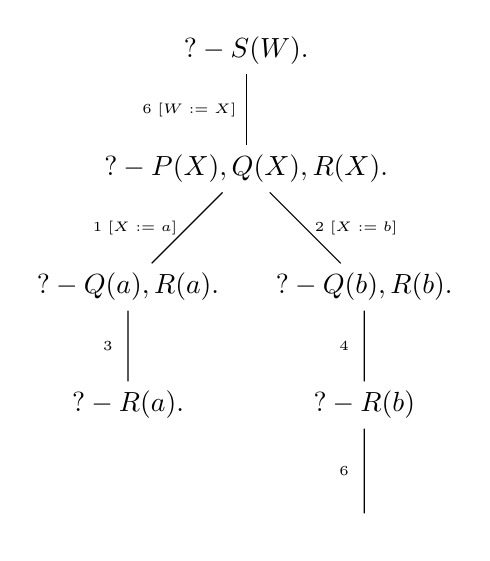
\begin{tikzpicture}
  \tikzstyle{level 1}=[sibling distance=25mm]
  \tikzstyle{level 2}=[sibling distance=30mm]
 
  \node {$?-S(W).$} 
  child { node {$?-P(X),Q(X),R(X).$}
      child {node {$?-Q(a),R(a).$}
	child { node {$?-R(a).$} edge from parent node [left] {\tiny $3 \;$} } edge 
from parent node [left] {\tiny $1 \; [X:=a]$}} 
      child {node {$?-Q(b),R(b).$} 
	child {node {$?-R(b)$} 
		child { node {$\cv$} edge from parent node [left] {\tiny $6 \;$} }  
edge 
from parent node [left] {\tiny $4 \;$}  } edge from parent node [right] {\tiny 
$ 
2 \; [X:=b]$}}
     edge from parent node [left] {\tiny $6 \;[W:=X]$} };
 \end{tikzpicture}
 \end{small}
\caption{Árbol SLD para la meta $\mathtt{?-S(W)}$.}
\end{minipage}
\hspace{1.3cm}
\begin{minipage}{.4\textwidth}
\centering
\begin{small}
 \begin{tikzpicture}
  \matrix (m) [matrix of math nodes, row sep=3em,
    column sep=1em]{
    ?-S(Y).&  S(X):-P(X),Q(X),R(X). \\
     ?-P(X),Q(X),R(X).& P(a). \\
    ?-Q(a),R(a).& Q(a).  \\
    ?- R(a). &  \\};
  \path[-]
    (m-1-1) edge (m-2-1) 
    (m-1-2) edge (m-2-1)
    (m-2-1) edge (m-3-1)
    (m-2-2) edge (m-3-1)
    (m-3-1) edge (m-4-1)
    (m-3-2) edge (m-4-1);
\end{tikzpicture}
\end{small}
\caption{SLD derivación para $\mathtt{?- S(Y)}$.}
\end{minipage}
\end{figure}

\begin{figure}[h!]
\centering
\begin{small}
 \begin{tikzpicture}
  \matrix (m) [matrix of math nodes, row sep=3em,
    column sep=1em]{
    ?-S(Y).&  S(X):-P(X),Q(X),R(X). \\
     ?-P(X),Q(X),R(X).& P(b). \\
    ?-Q(b),R(b).& Q(b).  \\
    ?- R(b). & R(b).  \\
    \cv & \\};
  \path[-]
    (m-1-1) edge (m-2-1) 
    (m-1-2) edge (m-2-1)
    (m-2-1) edge (m-3-1)
    (m-2-2) edge (m-3-1)
    (m-3-1) edge (m-4-1)
    (m-3-2) edge (m-4-1)
    (m-4-1) edge (m-5-1)
    (m-4-2) edge (m-5-1);
\end{tikzpicture}
\end{small}
\caption{SLD refutación para $\mathtt{?- S(Y).}$}
\end{figure}
\eeje

\beje
Considera el siguiente programa que describe el estilo de programaci\'on en el 
que est\'a basado un lenguaje de programaci\'on y los gustos de algunas 
personas por ciertos estilos. El \'arbol SDL corresponde a la meta 
$\mathtt{?-likes(X,scala).}$

\begin{small}
\[
 \begin{array}{rl}
  1. & \mathtt{based(prolog,logic).} \\
  2. & \mathtt{based(java,object).} \\
  3. & \mathtt{based(haskell,functional).} \\ 
  4. & \mathtt{based(scala,object).} \\
  5. & \mathtt{based(scala,functional).} \\\\
  6. & \mathtt{likes(max,logic).} \\
  7. & \mathtt{likes(hugo,object).} \\
  8. & \mathtt{likes(claire,functional).}\\
  9. & \mathtt{likes(X,L):- based(L,Y),likes(X,Y).}
 \end{array}
\]
\end{small}

\begin{center}
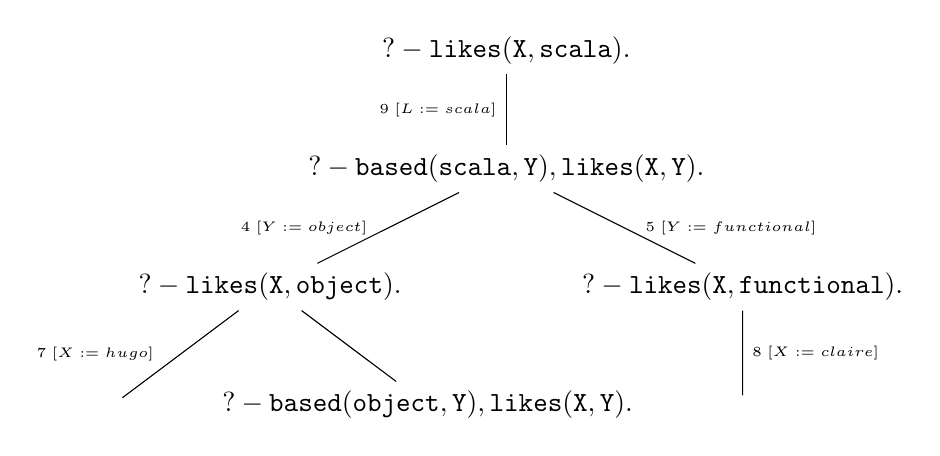
\begin{tikzpicture}
  \tikzstyle{level 1}=[sibling distance=75mm]
  \tikzstyle{level 2}=[sibling distance=60mm]
  \tikzstyle{level 3}=[sibling distance=40mm]
 
  \node {$\mathtt{?-likes(X,scala).}$} 
  child { node {$\mathtt{?-based(scala,Y),likes(X,Y).}$}
      child { node {$\mathtt{?-likes(X,object).}$}
         child { node {$\cv$} edge from parent node [left] {\tiny $7 
\;[X:=hugo]\;\;\;$} }
         child { node {$\mathtt{?-based(object,Y),likes(X,Y).}$} 
                    edge from parent node [left] {}}
      edge from parent node [left] {\tiny $4 \; [Y:=object]\;\;$}} 
      child {node {$\mathtt{?-likes(X,functional).}$} 
        child { node {$\cv$} edge from parent node [right] {\tiny $8 
\;[X:=claire]$} }   edge from parent node [right] {\tiny $\;\; 5 \; 
[Y:=functional]$}}
     edge from parent node [left] {\tiny $9 \;[L:=scala]$} };
\end{tikzpicture}
\end{center}
\eeje


\section{Sem\'antica de programas l\'ogicos}

Una parte importante de cada paradigma de programaci\'on es la
sem\'antica, por medio de la cual se le da significado a un programa,
situaci\'on que nos permite describir formalmente lo que \'este calcula.
Al inicio de esta nota mencionamos una ventaja de la programación declarativa: 
la elegancia matem\'atica resultado de la descripci\'on del programa mediante 
enunciados precisos, as\'i el significado del programa es claro y facilita su 
verificaci\'on.

\medskip

En esta secci\'on trataremos brevemente con dos clases de sem\'antica para 
programas l\'ogicos: la declarativa y la procedimental u operacional.


Comencemos observando que una cl\'ausula \verb=P :- Q1,Q2,...,Qn= de 
{\pl} tiene una interpretaci\'on declarativa y una interpretaci\'on 
procedimental:
\bi
 \item Declarativa: $P$ es v\'alida si $Q_1$ y $Q_2$ y $\ldots$ y
  $Q_n$ son v\'alidas.\\
  La interpretaci\'on declarativa permite discutir la correctud de
    la cl\'ausula.
 \item Operacional: Para ejecutar (probar) $P$ basta ejecutar $Q_1$ y $Q_2$ y 
  $\ldots$ y $Q_n$. \\
  La interpretaci\'on operacional permite considerar a la cl\'ausula como 
  la definici\'on de un proceso. Esta sem\'antica Se genera con la     
  ejecuci\'on del programa mediante las estrategias de control del int\'erprete 
  de {\pl}.
\ei

Una pregunta importante es si ambas interpretaciones generan la misma
informaci\'on, para contestarla necesitamos hablar del concepto de
respuesta de manera formal.

\defin{[Respuesta] Sean $\P$ un programa l\'ogico y $G=\meta G_1,\ldots,G_m$ una
  meta. Una respuesta para $\P\cup\{G\}$ es una sustituci\'on $\sigma$ tal que
  $Var(G_1)\cup\ldots\cup Var(G_m)\inc\mathsf{dom}(\sigma)$, es decir una
  sustituci\'on que incluye a las variables de $G$.
}

\defin{[Respuesta correcta] Decimos que una respuesta 
$\sigma$ para $\P\cup\{G\}$ es correcta si $\P\models G_i\sigma$ para toda
$1\leq i\leq m$, o equivalentemente si $\fa\P\models
\fa\big((G_1\land\ldots\land G_m)\sigma\big)$.
}

Recordemos que $\fa\vp$ denota a la cerradura universal de $\vp$ obtenida 
cuantificando universalmente todas las variables libres de $\vp$. 
An\'alogamente $\fa\P$ se obtiene de  $\P$ al cuantificar universalmente todas 
las variables de cada una de sus cl\'ausulas. Intuitivamente una respuesta
correcta para $\P\cup\{G\}$ corresponde a una consecuencia l\'ogica
particular del programa, y es entonces una significado declarativo del
programa. 

\beje Consid\'erese el programa
\[
\P=\{mq(0,suc(X)),\;mq(suc(Y),suc(X)\impp
mq(Y,X)\}.
\] 
Entonces $\sigma=[Y:=suc(suc(0))]$ es una respuesta
correcta para $?-mq(0,Y)$ pues 
\[
\fa\P\models mq(0,Y)[Y:=suc(suc(0))]
\]
\eeje

\defin{[Respuesta computada]Sean $\P$ un programa l\'ogico y $G$ una meta. Una 
sustituci\'on $\sigma$ es una respuesta computada para $\P\cup\{G\}$ si y 
s\'olo si existe una rama de \'exito en el \'arbol de SLD-resoluci\'on (o 
\'arbol de b\'usqueda) de longitud $n$ con unificadores m\'as generales
  $\mu_0,\ldots,\mu_{n-1}$ de tal forma que 
  $\sigma=\restr{\mu_0\mu_1\ldots\mu_{n-1}}{_{Var(G)}}$
}

Es decir $\sigma$ es una respuesta computada para $\P\cup\{G\}$ si y
s\'olo si $\sigma$ es la restricci\'on de la composici\'on de los unificadores 
de una rama de \'exito en el \'arbol de SLD-resoluci\'on para $\P\cup\{G\}$.

Intuitivamente una respuesta computada corresponde al resultado del proceso de 
inferencia por parte del sistema. Las respuestas computadas son aquellas que el 
int\'erprete de {\pl} devuelve al usuario. 

\beje
Si $\P=\{p(a),\;p(b),\;q(a),\;r(f(X))\impp p(X),q(X)\}$ entonces
tenemos la siguiente rama de \'exito en el \'arbol de SLD-resoluci\'on para la 
meta $G=\meta r(X)$:

\begin{small}
\begin{minipage}{.5\textwidth}
 \centering
 \[
 \begin{array}{rll}
  1. & p(a). & Hip. \\
  2. & p(b) & Hip. \\
  3. & q(a). & Hip. \\ 
  4. & r(f(Y))\impp p(Y),q(Y). & Hip.\\
  5. & \meta r(X) &Meta \\
  6. & \meta p(Y),q(Y) & SLDRes(4,5,[X:=f(Y)]) \\
  7. & \meta q(a)  & SLDRes(6,1,[Y:=a])\\
  8. & \cv. & SLDRes(3,7) 
 \end{array}
\]
\end{minipage}
\begin{minipage}{.5\textwidth}
\centering
  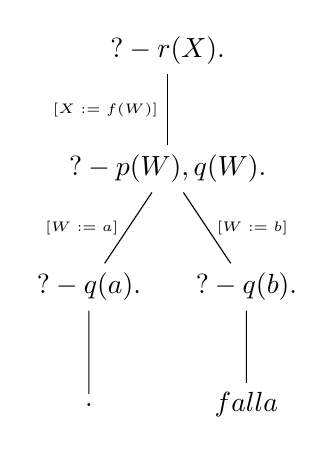
\begin{tikzpicture}
  \tikzstyle{level 1}=[sibling distance=35mm]
  \tikzstyle{level 2}=[sibling distance=20mm]
 
  \node {$?-r(X).$} 
  child { node {$?-p(W),q(W).$}
      child {node {$?-q(a).$}
	child { node {$\cv.$}} edge from parent node [left] {\tiny $[W:=a]$}} 
      child {node {$?-q(b).$} 
	child {node {$falla$}} edge from parent node [right] {\tiny $[W:=b]$}}
     edge from parent node [left] {\tiny $[X:=f(W)]$} };
 \end{tikzpicture}
\end{minipage}
\end{small}

La composici\'on de los unificadores es $[X:=f(a),Y:=a]$ de manera que 
la sustituci\'on $[X:=f(a)]$ es una respuesta computada para
$\P\cup\{\meta r(X)\}$.
\eeje

El significado de un programa l\'ogico se debe dar mediante sus respuestas, 
intuitivamente el significado es el conjunto de respuestas. Por ejemplo el 
siguiente programa $\mathbb{P}$, implementa la b\'usqueda de caminos en una 
gr\'afica:

\begin{alltt}
edge(a,b).
edge(b,c).
edge(b,d).
edge(c,d).
edge(e,f)
path(X,X).
path(X,Y) :- edge(X,Z),path(Z,Y).
\end{alltt}

De manera que el significado intensional de $\mathbb{P}$ es el conjunto de 
todos los caminos posibles (especificando todo los v\'ertices del camino) en la 
gr\'afica. Pero recordemos que la programaci\'on l\'ogica tiene un uso no 
est\'andar, por ejemplo el programa para concatenar dos listas, sirve tambi\'en 
para descomponer una lista en dos partes. Por lo que con esta definici\'on 
informal no es tan claro cu\'al es el significado. M\'as a\'un, dado un 
programa l\'ogico $\mathbb{P}$, podemos asignarle dos significados:
\begin{itemize}
 \item Significado declarativo: 
  el significado de un programa l\'ogico $\mathbb{P}$ es el conjunto de todas 
  las consecuencias l\'ogicas del programa, noci\'on asociada a la de respuesta 
  correctas.
 \item Significado operacional: 
  el significado de un programa l\'ogico $\mathbb{P}$ es el conjunto de todas 
  los \'exitos del programa, noci\'on asociada a la de respuesta computada.
\end{itemize}

Por supuesto que el significado deber\'ia ser \'unico,  pero no es claro que 
las dos nociones reci\'en enunciadas sean equivalentes. De los ejemplos 
anteriores se observa que una respuesta correcta tambi\'en es una respuesta 
computada y viceversa, ?`es esto v\'alido en general?, es decir ?`Toda
respuesta correcta puede computarse? y ?`Toda respuesta computada es
correcta? esto ayudar\'a a probar que las dos sem\'anticas coinciden.  \\
Resulta que en efecto ambos conceptos resultan equivalentes de cierta manera. 
Los enunciados formales para esta equivalencia, as\'i como su demostraci\'on 
requieren de conceptos como los modelos de Herbrand o sint\'acticos.
%M�s a�n, los dos conceptos de sem�ntica son satisfactorios desde el punto de 
% vista matem�tico pero no desde la perspectiva computacional, donde no nos 
% conformamos con conocer la definici\'on sino que requerimos en la medida de 
% lo posible de un algoritmo para calcularla. 

\section{Universo y Modelos de Herbrand}

\defin{[Universo de Herbrand] Sea $\L$ un lenguaje de primer orden. El universo 
de Herbrand de $\L$ se define como el conjunto $\H_\L$ de los t\'erminos 
cerrados de $\L$. Es decir
$$ \H_\L=\{t\mid t\text{ es un } \L\text{-t\'ermino cerrado }\} $$
}
\ejem{\hfill
\be
\item Si $\L_1=\{a,b, P^{(1)},Q^{(1)},R^{(2)}\}$ entonces 
$\;\H_{\L_1}=\{a,b\}$
\item Si $\L_2=\{c,a,f^{(1)},g^{(1)}, P^{(1)}\}$ entonces\\
$ \H_{\L_2}=\{c,a,f(c),f(a),g(c),g(a),f(f(a)),f(g(a)),f(f(c)),f(g(c)),g(g(a)),
g(g(c)),\ldots\} $
\ee
}

Obs\'ervese que si el lenguaje NO contiene s\'imbolos de funci\'on entonces el
universo de Herbrand es finito y es simplemente el conjunto de s\'imbolos de 
constante. 
Por otro lado si el lenguaje contiene al menos un s\'imbolo de funci\'on y un 
s\'imbolo de constante el universo de Herbrand se vuelve infinito. Si en un
lenguaje no hubiera constantes se agrega una para poder formar el universo de 
Herbrand.

\defin{[Base de Herbrand]
Sean $\L$ un lenguaje y $\H_\L$ su universo de Herbrand. La base de Herbrand 
$\B_\L$ de $\L$ se define como el conjunto de f\'ormulas at\'omicas cerradas, 
es decir, el conjunto de f\'ormulas at\'omicas cuyos argumentos pertenecen al 
universo de Herbrand de $\L$.
}

\ejem{Con respecto a los lenguajes del ejemplo anterior se tiene
\be
\item $\B_{\L_1}=\{Pa,Pb, Qa,Qb,Raa,Rbb, Rab, Rba\}$
\item 
  $\B_{\L_2}=\{Pc,Pa,Pfc,Pfa,Pgc,Pga,Pffa,Pfga,Pffc,Pfgc,Pgga,Pggc,\ldots\}$
\ee
}

\smallskip

En particular nos interesar\'a construir el universo y base de Herbrand de un 
programa l\'ogico, definidos como sigue: 
\vspace*{-5pt}
\defin{Dado un programa l\'ogico $\P$ definimos el universo $\H_\P$  y la
base de Herbrand $\B_\P$ de $\P$ como:
\[
\H_\P=_{def}\H_{\L(\P)}\qquad \qquad \B_\P=_{def}\B_{\L(\P)}
\]
 donde $\L(\P)$ es el lenguaje de los s\'imbolos de constante,
 funci\'on y predicado que figuran en $\P$.
}



\beje
Si $\P=\{nat(0).,\;nat(s(X))\impp nat(X).\}$ entonces
$\L(\P)=\{nat^{(1)},0,s^{(1)}\}$ y
\[
\H_\P=\{0,s(0),s(s(0)),\ldots\}\;\;\;\;\;\B_\P=\{nat(0),nat(s(0)),nat(s(s(0))),
\ldots\}
\]
\eeje


\beje
Si $\P$ es el programa l\'ogico para caminos en una gr\'afica (como en la nota 
11) entonces el lenguaje de $\P$ es $\L(\P)=\{a,b,c,d,e,f, edge^{(2)}, 
path^{(2)}\}$ y
$ \H_\P=\{a,b,c,d,e,f\} $
\[
\B_\P=\{edge(a,a),edge(a,b)\ldots, edge(f,e), edge(f,f),
path(a,a),path(a,b)\ldots,path(f,e),path(f,f)\}
\]
\eeje


\defin{[Interpretaci\'on de Herbrand]Decimos que una interpretaci\'on
$\M=\pt{M,\I}$ de un lenguaje dado $\L$ es una interpretaci\'on o modelo
de Herbrand si y s\'olo si se cumple lo siguiente:
\be
\item $M =\H_\L$ es decir, el universo de $\M$ es el universo de Herbrand de
  $\L$.
\item Para todo s\'imbolo de constante $c$, se cumple $\I(c)=c$.
\item Para todo s\'imbolo de funci\'on $f^{(n)}$, se cumple
  $\I(f(t_1,\ldots,t_n))=f(t_1,\ldots,t_n)$.
\item Para todo s\'imbolo de predicado $P^{(n)}$ es un subconjunto de 
$P^\N\inc\H_\L^n$
\ee
}

Obs\'ervese que en una interpretaci\'on de Herbrand los s\'imbolos de constante 
y de funci\'on se interpretan como ellos mismos y que lo \'unico que no est\'a
determinado es la interpretaci\'on de los s\'imbolos de predicado por esta
raz\'on a los modelos de Herbrand tambien se les llama modelos sint\'acticos.


\subsection{Representaci\'on de modelos de Herbrand}

Una manera \'util de representar modelos de Herbrand es mediante subconjuntos de
la base de Herbrand del lenguaje en cuesti\'on. Dado un modelo de Herbrand 
$\M$, representamos a $\M$ mediante el subconjunto $B_\M\inc\B_\H$ de aquellas 
f\'ormulas at\'omicas que son verdaderas en $\M$. De esta manera, si la base es 
finita, es posible construir todos los modelos de Herbrand, y en el caso en que 
la base es infinita el n\'umero de modelos de Herbrand tambi\'en, pero pueden 
enumerarse efectivamente como subconjuntos de la base.

\beje
Si $\mathcal{L}=\{a, P^{(1)},Q^{(1)}\}$ entonces 
\[
\H_\L=\{a\}\;\;\;\;\B_\L=\{Pa,Qa\}
\]
y existen cuatro interpretaciones o modelos de Herbrand para $\L$:
\begin{enumerate}
\item $\M_1$ tal que $\M_1\models Pa$ y $\M_1\models Qa$
\item $\M_2$ tal que $\M_2\models Pa$ y $\M_2\not\models Qa$
\item $\M_3$ tal que $\M_3\not\models Pa$ y $\M_3\models Qa$
\item $\M_4$ tal que $\M_4\not\models Pa$ y $\M_4\not\models Qa$
\end{enumerate}
Cada modelo corresponde a un subconjunto $B_{\M_i}$ de la base como sigue:
\begin{enumerate}
\item $B_{\M_1}=\B_\L=\{Pa,Qa\}$ representa a $\M_1$
\item $B_{\M_2}=\{Pa\}$ representa a $\M_2$
\item $B_{\M_3}=\{Qa\}$ representa a $\M_3$
\item $B_{\M_4}=\varnothing$ representa a $\M_4$

\end{enumerate}
\eeje

Dado que cada subconjunto de $B\inc \B_\L$ determina de manera \'unica a un 
modelo de Herbrand $\M$,  identificamos a $\M$ con $B$. Por ejemplo, el modelo 
$\M_2$ del ejemplo anterior, se define como $\M_2=\{Pa\}$.
% \beje
% Consid\'erese el siguiente programa
% \begin{verbatim}
%   alumno(A,P) :- estudia(A,C), ensea(P,C).
%   estudia(ana,logica).
%   estudia(ana,algebra).
%   estudia(eva,algoritmos).
%   ensea(juan,logica).
%   ensea(juan,algebra)
%   ensea(carlos,algoritmos) 
% \end{verbatim}

Con esta idea en mente, si deseamos verificar que una f\'ormula at\'omica 
$A$ es verdadera en $\M$ basta ver que  $A\in B_\M$ 
% aunque usualmente abusamos de la notaci\'on usando $\M$ en vez de
% $B_\M$, es decir escribimos $A\in\M$. 

El siguiente lema nos dice c\'omo se evaluan los t\'erminos en una 
interpretaci\'on de Herbrand:

\lema{Sean $\L$ un lenguaje, $\M=\pt{M,\I}$ una interpretaci\'on de Herbrand 
para $\L$, $t$ un t\'ermino con variables $x_1,\ldots,x_n$ y $\nu$ un estado de 
las variables tal que $\nu(x_i)=r_i$ donde $r_i\in\H_\L$ es decir, $r_i$ es un 
t\'ermino cerrado, para cada $1\leq i\leq n$. Entonces: 
\[
\I_\nu(t)=t[x_1:=r_1,\ldots,x_n:=r_n]
\]
En particular si $t$ es un t\'ermino cerrado entonces $\I_\nu(t)=t$
}
\proof (Por inducci\'on sobre los t\'erminos). Ejercicio.\qed


\espc

El lema anterior nos dice que la interpretaci\'on de t\'erminos en un
modelo de Herbrand coincide con aplicar una sustituci\'on al t\'ermino
y que los t\'erminos cerrados se interpretan como ellos mismos.

% \defin{Sean $\vp$ una f\'ormula y $\sigma$ una sustituci\'on, decimos que
% $\vp\sigma$ es una instancia cerrada de $\vp$ si $\vp\sigma$ no
% contiene variables libres.
% }


\section{El Teorema de Herbrand}


El teorema de Herbrand es esencial para describir la sem\'antica de
programas l\'ogicos, a continuaci\'on lo estudiamos con detalle.

\defin{Sean $\L$ un lenguaje y $\K$ un conjunto de $\L$-f\'ormulas cerradas y 
universales. El conjunto de instancias cerradas $\vp\sigma$ o cerraduras 
universales, donde~$\fa x_1\ldots\fa x_n\vp\;$ pertenece a $\K$, se llama 
conjunto de instancias 
cerradas de $\K$ y se denota $IC(\K)$.
}
%Obs\'ervese que en realidad $IC(\K)=\{Cl(\chi)\sigma\mid\chi\in \K\;\mbox{y}
%\; Cl(\chi)\sigma\;\mbox{es una instancia cerrada}\}$ es decir el
%conjunto de instancias cerradas de $\K$ coincide con el conjunto de instancias
%cerradas de la forma clausular de cada f\'ormula de $\K$.
%%\bigskip\\ 
A continuaci\'on presentamos el Teorema Cl\'asico de Herbrand enunciado de 
forma adecuada a nuestras necesidades.
\teo{[de Herbrand]Sean $\L$ un lenguaje con al menos una constante y $\K$ un 
conjunto de $\L$-enunciados universales. Las siguientes condiciones son 
equivalentes:
\be
\item $\K$ tiene un modelo.
\item $\K$ tiene un modelo de Herbrand.
\item $IC(\K)$ tiene un modelo.
\item $IC(\K)$ tiene un modelo de Herbrand. 
\ee
}
\proof
Debido a que todo modelo de Herbrand es un modelo, las implicaciones
$b\Imp a$ y $d\Imp c$ son triviales.\\ La v\'alidez universal de la
f\'ormula $\fa x_1\ldots\fa x_n\vp\imp \vp\{x_1/t_1,\ldots,x_n/t_n\}$ hace
inmediatas a las implicaciones $a\Imp c$ y $b\Imp d$. 
As\'{\i} que basta probar la implicaci\'on $c\Imp b$.  \\
Sea $\M$ un modelo de $IC(\K)$. Definimos una estructura de Herbrand 
$\mathcal{N}=\pt{\H_\L,\I}$, para lo cual basta decir como se interpretan los 
s\'{\i}mbolos de predicado, puesto que por definici\'on los s\'{\i}mbolos de 
constante y de funci\'on se interpretan como ellos mismos. Si $P$ es un 
s\'{\i}mbolo de predicado $n$-ario, entonces definimos:  
$$P^\mathcal{N}=\{(t_1,\ldots,t_n)\mid \M\models P(t_1,\ldots,t_n) \} $$  
Obs\'ervese que, por construcci\'on de $\mathcal{N}$, se cumple que: 
$$
\M\models P(t_1,\ldots,t_n)\;\text{si  y s\'olo si } \mathcal{N}\models 
P(t_1,\ldots,t_n)
$$
es decir, $\M$ y $\mathcal{N}$ validan a las mismas f\'ormulas at\'omicas
cerradas. Dicho resultado se puede extender a cualquier f\'ormula cerrada
libre de cuantificadores mediante inducci\'on sobre f\'ormulas 
(ejercicio~\footnote{Hay que probar el siguiente \begin{lemma}Si $\vp$ es un 
enunciado sin cuantificadores entonces $\M\models\vp$ syss 
$\Nc\models\vp$.\end{lemma}}).
\\ Por \'ultimo veamos que $\mathcal{N}$ es modelo de $\K$. Sea $\fa 
x_1\ldots\fa
x_n\vp$ una f\'ormula de $\K$. Queremos demostrar que $\mathcal{N}\models\fa
x_1\ldots\fa x_n\vp$, lo cual es equivalente a mostrar que para cualesquiera 
$t_1,\ldots,t_n\in\;\H_\L,\;\;\mathcal{N}\models\vp[x_1:=t_1,\ldots,x_n:=t_n]$. 
Pero esta \'ultima afirmaci\'on es equivalente, por lo reci\'en observado a que
para cualesquiera
$t_1,\ldots,t_n\in \H_\L,\;\;\M\models\vp[x_1:=t_1,\ldots,x_n:=t_n]$,
lo cual es cierto puesto que $\vp[x_1:=t_1,\ldots,x_n:=t_n]$ pertenece a
$IC(\K)$ y por hip\'otesis, $\M$ es modelo de $IC(\K)$. De manera que 
$\mathcal{N}\models\fa x_1\ldots\fa x_n\vp$ por lo que $\mathcal{N}$ es un 
modelo de Herbrand de $\K$.\qed 


\medskip

Es importante observar que el teorema de Herbrand s\'olo es v\'alido para
enunciados universales. Por ejemplo si 
$\K=\{Pa,\ex x \neg Px\}$ entonces $\K$ es un conjunto de f\'ormulas cerradas
pero no universales y claramente tiene un modelo, digamos
$M=\{0,1\}$ con $\I(a)=0$ y $P^\M=\{0\}$, pero $\K$ no tiene un modelo de 
Herbrand pues el universo de Herbrand es $\H_\L=\{a\}$ de manera que los 
\'unicos modelos de Herbrand son los representados por $\vacio$ que corresponde 
a una  interpretaci\'on donde $Pa$ es falsa y por lo tanto no es modelo de 
$\K$; y el representado por $\{Pa\}$ que tampoco es modelo de $\K$ pues $\ex 
x\neg Px$ es falsa.

\smallskip

Dado que las cl\'ausulas son enunciados universales, se tiene el siguiente
\vspace*{-5pt}
\begin{corollary}
Sea $\mathcal{C}$ un conjunto de cl\'ausulas de Horn. Las siguientes 
condiciones son equivalentes:
  \begin{itemize}
  \item $\mathcal{C}$ tiene un modelo.
  \item $\mathcal{C}$ tiene un modelo de Herbrand.
  \end{itemize}
\end{corollary}

\noindent En lo que resta de esa nota presentamos algunos resultados 
sem\'anticos para programas l\'ogicos de Horn. 


\subsection{Sem\'atica declarativa de programas l\'ogicos}

Debido a las formas de sus cl\'ausulas, un programa l\'ogico~$\P$ siempre
tiene un modelo en particular debido al teorema de Herbrand basta
estudiar los modelos de Herbrand del programa~$\P$. El significado
declarativo del programa~$\P$ consiste de todas las consecuencias
l\'ogicas de~$\P$ y puede representarse con un modelo particular llamado
el modelo m\'inimo de Herbrand de $\P$.

% \defin{Dado un programa l\'ogico $\P$ decimos que la interpretaci\'on
%   $\M=\pt{M,\I}$ es un modelo de $\P$ si $\M$ es modelo de la cerradura
%   universal $\fa\C$ de $\C$ para toda cl\'ausula $\C\in\P$.
% }

% \teo{[de Herbrand para Programas Lgicos] Sean $\P$ un programa l\'ogico y
% $\M$ un modelo de $\P$. El conjunto $\M_\H=\{R\in\B_\P\mid\M\models R\}$ 
% representa a un modelo de  Herbrand de $\P$
% }
% Este resultado nos permite construir un modelo de Herbrand para un programa
% l\'ogico a partir de un modelo dado.


Construir la base de Herbrand de $\P$ es importante debido a la siguiente

\prop{Si $\P$ es un programa l\'ogico entonces $\P$ tiene un modelo de
  Herbrand}
% cuya representacin es $\B_\P$ la base de Herbrand de $\P$.
\proof
La base de Herbrand $\B_\P$ representa al modelo que hace verdaderas a todas
las f\'ormulas at\'omicas del lenguaje lo cual implica que todas las cl\'ausulas
de $\P$ son verdaderas debido a su forma (hechos o reglas). 
\qed

\medskip

De manera que cualquier programa l\'ogico tiene al menos un modelo de Herbrand, 
enseguida veremos que existe un modelo de Herbrand m\'inimo con respecto a la 
contenci\'on.
\prop{Sea $\P$ un programa l\'ogico. $\P$ tiene un modelo de Herbrand m\'inimo
  $\M_\P$ definido por:
%\[
\[
\M_\P=\bigcap\{\M\mid\M\;\mbox{ es modelo de Herbrand de }\;\P\}
\]
%\M_\P=\{G\in\B_\P\mid\P\models G\}
%\]
}
\proof
Sabemos que $\P$ tiene al menos un modelo de Herbrand representado por
la base de Herbrand $\B_\P$. Es f\'acil ver que si $\M_1,\M_2$ son modelos de 
Herbrand de $\P$ su intersecci\'on tambi\'en lo es. De manera que el modelo 
m\'inimo de Herbrand $\M_\P$ est\'a bien definido.
\qed

\prop{Sea $\P$ un programa l\'ogico. El modelo de Herbrand m\'inimo
  $\M_\P$ se representa con el conjunto de \'atomos que son consecuencia
  l\'ogica de $\P$. Es decir, %puede definirse como
\[
\M_\P=\{A\in\B_\P\mid\P\models A\}
\]
}
\proof
$\inc).$ Sea $A\in\M_\P$. Veamos que $\P\models A$. Si esto no sucediera 
entonces $\P\cup\{\neg A\}$ tendr\'ia un modelo y por el teorema de Herbrand 
tendr\'ia un modelo de Herbrand $\Nc$. Pero entonces como $\Nc\models\neg A$ 
mos que $A\notin\Nc$ pero por minimalidad  $\M_\P\inc\Nc$ y entonces 
tambi\'en $A\in\Nc$ lo cual es absurdo.\\
$\supseteq).$ Sea $A$ tal que $\P\models A$. Queremos ver que $A\in\M_\P$. Como 
$\M_\P$ es modelo de $\P$ y $\P\models A$ entonces $\M_\P\models A$, es decir, 
$A\in\M_\P$.
%Basta ver que el conjunto $\{A\in\B_\P\mid\A\models G\}$ representa a un 
% modelo de Herbrand de $\P$.
% \proof
% Sabemos que $\P$ tiene al menos un modelo de Herbrand. Es f\'acil ver
% que si $\M_1,\M_2$ son modelos de Herbrand de $\P$ su intersecci\'on
% tambi\'en lo es. De manera que el modelo m\'inimo de Herbrand existe y se
% define como
% \[
% \M_\P=\bigcap\{\M\mid\M\;\mbox{ es modelo de Herbrand de }\;\P\}
% \]
% \qed
% $\M_\P$ es el conjunto de todas las consecuencias l\'ogicas de $\P$. De hecho 
% $\M_\P$ es la intersecci\'on de todos los
% modelos de Herbrand de $\P$.\\

\medskip

Dado que $\M_\P$ contiene exactamente a todos los \'atomos que son 
consecuencia
l\'ogica de $\P$ entonces este modelo corresponde realmente al significado
intensional o estandar de $\P$. Es decir, la sem\'antica declarativa de $\P$ 
est\'a dada por $\M_\P$.


\subsection{Procedimiento para hallar el modelo m\'inimo de Herbrand}

Desde el punto de vista puramente matem\'atico la sem\'antica declarativa de un
programa l\'ogico ha quedado definida mediante el modelo m\'inimo. Sin embargo, 
en la pr\'actica no es claro c\'omo construir directamente a $\M_\P$, pues su
definici\'on involucra a una intersecci\'on generalmente infinita. A 
continuaci\'on veremos que existe una manera \textbf{mec\'anica} para construir 
el modelo m\'inimo.

\defin{Dado un programa l\'ogico $\P$, el operador de
  consecuencia inmediata $\T_\P$ se define como sigue
\[
\T_\P(\K)=\{P\in\B_\P\mid P\impp Q_1,\ldots,Q_m\;\mbox{es instancia cerrada de 
una   cl\'ausula de } \P \mbox{ y } Q_1,\ldots,Q_m\in\K\}
\]
donde $\K\inc\B_\P$. %es un modelo de Herbrand para $\P$.
}


\defin{Sea $\P$ un programa l\'ogico. Definimos las iteraciones del
  operador de consecuencia inmediata~$\T_\P$ para $\K\inc\B_\P$ recursivamente  
como sigue:
\[
\ba{rll}
\T_0(\K) & = & \K \\ \\
\T_{n+1}(\K) & = & \T_\P\big(\T_n(\K)\big) \\ \\
% \R_n(\P)\cup \T_\P\big(\R_n(\P)\big) \\ \\
\T_\omega(\K) & = & \bigcup_{n=0}^\infty\T_n(\K)
\ea
\]
}


El modelo m\'inimo de Herbrand de un programa l\'ogico puede obtenerse mediante
las iteraciones del operador de consecuencia inmediata iniciando en el
conjunto vac\'io, como lo asegura la siguiente

\prop{Sean $\P$ un programa l\'ogico y $\M_\P$ su m\'inimo modelo de Herbrand. 
Entonces $\M_\P=\T_\omega(\vacio)$.
}
% \teo{Sean $\P$ un programa l\'ogico y  $\vp=\ex x_1\ldots\ex 
% x_n(Q_1\land\ldots
% \land Q_m)$ una f\'ormula existencial cerrada. 
% Las siguientes condiciones son equivalentes:
% \bi
% \item $\P\models\vp$.
% \item $\P\models(Q_1\land\ldots\land Q_m)[x_1,\ldots,x_n:=t_1,\ldots,t_n]$ 
% para
%   algunos $t_1,\ldots,t_n\in\H_\P$.
% \item $\M_\P$ es un modelo de $\vp$.
% \item $\M_\P\models(Q_1\land\ldots\land Q_m)[x_1,\ldots,x_n:=t_1,\ldots,t_n]$
%   para algunos $t_1,\ldots,t_n\in\H_\P$.
% \ei
% }

% La importancia del teorema anterior se resalta al considerar el problema
% fundamental de la programacin l\'ogica:\\
% Dado un programa l\'ogico $P$ y una consulta $Q_1,\ldots,Q_m$ nos preguntamos 
% si
% $\P\models Q_1,\ldots,Q_m$ o equivalentemente si $\P\cup\{?-Q_1,\ldots,Q_m\}$
% no tiene modelo. Obs\'ervese que la cl\'ausula meta$?-Q_1,\ldots,Q_m$ es lo 
% mismo que
% $\pmi Q_1,\ldots,Q_m\equiv\neg(Q_1\land\ldots\land Q_m)$ cuya
% cerradura universal es $\fa x_1\ldots x_n(\neg(Q_1\land\ldots\land Q_m))$ que
% es una f\'ormula universal equivalente a $\neg\exists x_1\ldots
% x_n(Q_1\land\ldots\land Q_m)$. De manera que el problema original se deduce a
% decidir si $\P\models\ex x_1\ldots x_n(Q_1\land\ldots\land Q_m)$. Si
% realmente se da este caso por el teorema anterior tal consecuencia es
% atestiguada por una serie de instancias concretas para las variables
% $x_1,\ldots,x_n$ mediante t\'erminos cerrados $t_1,\ldots,t_n$. M\'as a\'un 
% tales
% t\'erminos cerrados pueden obtenerse analizando al m\'inimo modelo de Herbrand
% $\M_\P$. Por lo que $\M_\P$ es realmente el \emph{significado} del programa
% l\'ogico $\P$.


% El siguiente resultado aclara el concepto de respuesta correcta al decirnos
% que las respuestas correctas son el tipo de respuesta que esperariamos obtener
% al hacernos preguntas existenciales.

% \prop{Sea $\P$ un programa l\'ogico. Se cumple lo siguiente:
% \bi
% \item Sea $G= ?-G_1,\ldots,G_m$ una meta con variables
%   $y_1,\ldots,y_k,x_1,\ldots,x_n$. Si \[\P\models \fa y_1\ldots\fa y_k\ex
%   x_1\ldots\ex x_n(G_1\land\ldots\land G_m)\]
%  entonces existe una respuesta
%   correcta $\sigma$ para $\P\cup\{G\}$ tal que
%   $\sigma=[x_1:=t_1,\ldots,x_n:=t_n ]$ donde los t\'erminos $t_1,\ldots,t_n$
%   contienen s\'olo variables del conjunto $\{y_1,\ldots,y_k\}$.
% \item Inversamente sean $G= ?-G_1,\ldots,G_m$ una meta y
% $\sigma=[x_1:=t_1,\ldots,x_n:=t_n ]$ una respuesta correcta para
% $\P\cup\{G\}$ donde los t\'erminos $t_1,\ldots,t_n$
%   contienen s\'olo variables del conjunto $\{y_1,\ldots,y_k\}$. Si
% $y_1,\ldots,y_k,x_1,\ldots,x_n$ son variables distintas entonces 
% \[\P\models \fa y_1\ldots\fa y_k\ex
%   x_1\ldots\ex x_n(G_1\land\ldots\land G_m)\]
% \ei
% }

% La pregunta que surge inmediatamente es ?`c\'omo calcular respuestas
% correctas? lo cual responderemos mediante la sem\'antica operacional de
% los programas l\'ogicos.


Veamos un ejemplo.

\beje
Sea $\P$ el siguiente programa $\{p(X,a)\impp q(X).\; p(X,Y)\impp q(X),r(Y). 
\; q(a). \; r(b). \; q(b). \; r(c). \}$
\bi
\item El lenguaje de $\P$ es $\L(\P)=\{a,b,c,p^{(2)},q^{(1)},r^{(1)}\}$
\item El universo de Herbrand de $\P$ es $\H_\P=\{a,b,c\}$
\item La base de Herbrand de $\P$ es
\begin{small}
  \[\B_\P = \{  q(a),q(b),q(c),r(a),r(b),r(c),
               p(a,a),p(a,b),p(a,c), p(b,a),p(b,b),p(b,c), 
                p(c,a),p(c,b),p(c,c) \}\]
\end{small}
\item El modelo m\'inimo de Herbrand de $\P$ es:
\bi
\item $\T_0(\vacio)= \vacio$
\item $\T_1(\vacio)=
  \T_\P(\T_0(\vacio))=\T_\P(\vacio)=\{q(a),r(b),q(b),r(c)\}$
\item
  $\T_2(\vacio)=\T_\P(\T_1(\vacio))=\T_\P(\{q(a),r(b),q(b),r(c)\})$
\item[] 
$\;\;\;\;\;\;\;\;\;\;\;=\{q(a),r(b),q(b),r(c),p(a,a),p(b,a),p(a,b),p(a,c),p(b,b)
,p(b,c)\}$
\item $\T_3(\vacio)=\T_\P(\T_2(\vacio))=\T_2(\vacio)$
%\item $\T_4(\vacio)=\T_\P(\T_3(\vacio))=\T_\P(\vacio)$
\ei
\item En el paso $n=3$ la sucesi\'on se estabiliza y concluimos 
\[
\M_\P=\T_\omega(\vacio)=\{q(a),r(b),q(b),r(c),p(a,a),p(b,a),p(a,b),p(a,c),p(b,b)
,p(b,c)\}
\]
\ei
\eeje

\subsection{Sem\'atica operacional de programas l\'ogicos}


El significado operacional de un programa l\'ogico consiste en los
resultados obtenidos al ejecutar el programa. 

\defin{El conjunto de \'exito de un programa l\'ogico $\P$ se define como
\[
\mathcal{E}_\P=\{A\in\B_\P\mid\P\cup\{\normalfont{?-}A\}\;\mbox{tiene
    una SLD-refutaci\'on}\;\}\] 
}

\noindent
La sem\'antica operacional del programa $\P$ se define como el conjunto
de \'exitos $\mathcal{E}_\P$.  
Veamos un ejemplo

\beje
Sea $\P$ el siguiente programa $\{p(f(X))\impp p(X).,\; p(a).,\; q(b). \}$.
Entonces 
\bi
\item El lenguaje de $\P$ es $\L(\P)=\{a,b,p^{(1)},q^{(1)},f^{(1)}\}$
\item El universo de Herbrand de $\P$ es 
$\H_\P=\{a,b,f(a),f(b),f(f(a)),f(f(b)),\ldots\}$
\item La base de Herbrand de $\P$ es
  \[\B_\P  = \{  p(a),p(b),q(a),q(b),p(f(a)),p(f(b)),q(f(a)),q(f(b)),\ldots\}
\]

\item Claramente las metas $\normalfont{?-}p(a).$ y $\normalfont{?-}q(b).$ 
tienen una SLD-refutaci\'on por lo tanto pertenecen a $\mathcal{E}_\P$.
\item La meta $\normalfont{?-}p(f(a)).$ tiene \'exito pues tenemos una  
SLD-refutaci\'on a partir de las instancias $p(f(a))\impp p(a).$ y $p(a).$ de 
las cl\'ausulas del programa.
\item Similarmente podemos verificar que $\normalfont{?-}p(f^n(a)).$ tiene 
\'exito para cualquier $n\geq 0$. M\'as a\'un si una meta es \'exitosa entonces 
es de esta forma (salvo $?-q(b)$).
\item Por lo tanto el conjunto de \'exitos es:
\[
\mathcal{E}_\P=\{p(a),q(b)\}\cup\{p(f^n(a))\mid n\geq 1\}
\]
\ei
\eeje


\section{Equivalencia de ambas sem\'anticas}

Finalmente observamos la equivalencia de ambas sem\'anticas. Esta equivalencia 
es corolario de ciertos resultados te\'oricos que dependen del teorema de 
Herbrand. 

\begin{proposition}
Sea $\P$  un programa l\'ogico definido. La sem\'anticas declarativa y 
operacional para $\P$ coinciden. Es decir,
\[
\M_\P = \mathcal{E}_\P
\]
\end{proposition}

De manera que toda consecuencia l\'ogica at\'omica de $\P$ es un \'exito de 
$\P$ y viceversa, todo \'exito $G\in\mathcal{E}_\P$ es consecuencia l\'ogica de 
$\P$, es decir, cumple $\P\models G$.

% \teo{[Correctud de la SLD-resoluci\'on]
% Sean $\P$ un programa l\'ogico y $G=?-G_1,\ldots,G_m$ una meta. Cualquier
% respuesta computada $\sigma$ para $\P\cup\{G\}$ es una respuesta correcta
% para $\P\cup\{G\}$. M\'as a\'un si  $\sigma$ es una respuesta computada para
% $\P\cup\{G\}$ y $\tau$ es una sustituci\'on arbitraria entonces
% $\restr{\sigma\tau}{_G}$ es una respuesta correcta para $\P\cup\{G\}$.

% }

% \cor{Sean $\P$ un programa l\'ogico y $G=?-G_1,\ldots,G_m$ una meta. Si
%   existe una SLD-refutaci\'on de $\P\cup\{G\}$ entonces $\P\cup\{G\}$ no tiene
%   modelo y por lo tanto $\P\models\ex(G_1\land\ldots\land G_m)$.
% }

% \cor{
% $\mathcal{E}_\P\inc \M_\P$. Es decir cualquier \'exito pertenece al
% modelo m\'inimo de Herbrand de $\P$.
% }


% \teo{[Completud de la SLD-resoluci\'on] Sean $\P$ un programa l\'ogico y 
% $G=?-G_1,\ldots,G_m$ una meta. Si $\P\models\ex(G_1\land\ldots\land G_m)$
% entonces existe una SLD-refutaci\'on de $\P\cup\{G\}$.
% }


% \cor{$\M_\P\inc \mathcal{E}_\P$. Es decir, cualquier \'atomo
%   perteneciente al modelo m\'inimo de Herbrand de $\P$ pertenece a los
%   \'exitos de $\P$.}

% \teo{[Completud de la SLD-resoluci\'on con respecto a respuestas] 
% Sean $\P$ un programa l\'ogico, $G=?-G_1,\ldots,G_m$ una meta y $\sigma$ una
% respuesta correcta para $\P\cup\{G\}$. Entonces existe una respuesta
% computada $\mu$ para $\P\cup\{G\}$ y una sustituci\'on $\tau$ tales que
% $\sigma=\restr{\mu\tau}{_G}$. 
% }


\section{Incompletud e Incorrectud de {\pl}}

Debido a que las implementaciones de {\pl} no verifican las presencia de 
una variable en un t\'ermino en la unificiaci\'on de $\{X,t\}$ las propiedades 
de correctud completud no son v\'alidas como lo muestran los siguientes 
ejemplos:

\bi

\item Incorrectud: {\pl} contesta que \verb-true- a una meta que no es 
consecuencia l\'ogica del programa:
\begin{verbatim}
test :- p(X,X).

p(Y,f(Y)).

--------------------
?- test.
true.

?- p(X,X).
X = f(X).
\end{verbatim}

\item Incompletud: en el siguiente ejemplo \verb-q- es consecuencia l\'ogica 
del programa pero {\pl} se cicla y queda sin recursos sin poder contestar 
afirmativamente.
\begin{verbatim}
p :- q.
p :- r.
q :- p.
r.

--------------------------
?- q.
ERROR: Out of local stack
   Exception: (4,193,042) p ? abort
% Execution Aborted
?- 
\end{verbatim}

\ei



% %FIXME
\bibliographystyle{plain}
\bibliography{referencias}
\nocite*{}


\end{document}
